% -*- Mode:TeX -*-
% LaTeX template for CinC papers                   v 1.1a 22 August 2010
%
% To use this template successfully, you must have downloaded and unpacked:
\documentclass[twocolumn]{cinc}
\usepackage{amsmath, graphicx, xurl, hyperref}
\usepackage{caption}
\usepackage{python}
\usepackage{listings}
\usepackage{xcolor}
%\usepackage{amssymb}

\usepackage[utf8]{inputenc}
\usepackage{amssymb, latexsym}
 
\usepackage{tikz}
\usetikzlibrary{decorations.pathreplacing}
\usetikzlibrary{fadings}

\definecolor{codegreen}{rgb}{0,0.6,0}
\definecolor{codegray}{rgb}{0.5,0.5,0.5}
\definecolor{codepurple}{rgb}{0.58,0,0.82}
\definecolor{backcolour}{rgb}{0.95,0.95,0.92}

\lstdefinestyle{mystyle}{
    backgroundcolor=\color{backcolour},   
    commentstyle=\color{codegreen},
    keywordstyle=\color{magenta},
    numberstyle=\tiny\color{codegray},
    stringstyle=\color{codepurple},
    basicstyle=\ttfamily\footnotesize,
    breakatwhitespace=false,         
    breaklines=true,                 
    captionpos=b,                    
    keepspaces=true,                 
    numbers=left,                    
    numbersep=5pt,                  
    showspaces=false,                
    showstringspaces=false,
    showtabs=false,                  
    tabsize=2
}

\lstset{style=mystyle}

\title{Regression and Classification using Machine Learning and Deep Learning methods}
\author{Bjørn-Jostein Singstad \textsuperscript{1}\\ \ \\
\textsuperscript{1}University of Oslo, Oslo, Norway}

\begin{document}
\maketitle

\begin{abstract}

\textbf{Introduction}
The objective of this study was to develop, train and test a variety of different regression methods and classification methods. The aim was to employ the models on three different data sets (one for the regression tasks and two for classification) and compare the results.

\textbf{Method}
The three data sets used in this study was; (1) data generated by Franke's function, (2) Modified National Institute of Standards and Technology database (MNIST) hand written digits  and (3) Physikalisch Technische Bundesanstalt, Brunswick (PTB)-XL ECG database. The first data set, the data generated by Franke's function, was used for regression. The two other data set were used for classification.

The regression models developed in this study were;  OLS, Ridge regression, OLS with Stochastic Gradient Decent (SGD) optimizer and a Neural Network. The models were tested and validated using k-fold cross validation and selection was done based on the R2-score. 

The classification models were developed was a Neural Network and a Logistic regression algorithm. The models were tested and validated using different methods such as hold-out validation, k-fold cross validation and Bayesian hyper parameter tuning. Model selection was done using the accuracy score. 

\textbf{Results}
The OLS with SDG optimization and optimized hyper parameters got a cross validated  R2-score of ... and MSE of..... The performance n the test set was... The Ridge with SDG optimization and optimized hyper parameters got a cross validated  R2-score of ... and MSE of..... The performance n the test set was. .. The Neural Network used for regression got a cross validated  R2-score of ... and MSE of..... The performance n the test set was...

The Neural network employed on the classification performed an crossvalidatd accuracy score of ..  on the MNIST data and .. on the test set. The logistic regression that was used on the MNIST data got an cross validated accuracy score of ... and ... on the test set.
The Neural Network used for classification of the PTB-XL data set got a cross validated accuracy score of ... and a test score of ...
The logistic regression employed on the PTB-XL data set got a cross validated accuracy score of .... and a test score of ...

\textbf{Conclusion}
The results achived in this study shows that a ... outperforms ... and ... on data generated frm Frankes function when measuring the performance using R2-score and MSE score. The results from classifying the MNIST data shows that ... performs better than ... . On the other hand the ... outpeformed ... on the PTB-XL fata.

\end{abstract}
% LaTeX inserts the extra space here automatically.

\section{Introduction}
Regression and classification are two of the main topics in Machine Learning. A sub-field of machine learning is called deep learning, where more complex architectures of neural networks are better able to scale with the amount of data in terms of performance. The scope of this study is to train, test and compare a three different regression algorithms two classification algorithms based on both traditional machine learning algorithms and Deep Learning algorithms.

A previously developed ordinary least square (OLS) and Ridge regression algorithm\cite{bjorn-jostein_singstad_using_nodate} will be used a starting point and modified with a new Stochastic Gradient Decent (SGD) optimization algorithm. These two models will be compared with the original models, developed in  \cite{bjorn-jostein_singstad_using_nodate}, and new developed Neural Network. 

For the classification task the same Neural Network will be used, but with different activation functions and cost function. The neural network will be compared with a logistic regression algorithm based on the accuracy score on both the MNIST and PTB-XL ECG data set.

Three data sets will be used for training and validation. The first data set, which is going to be used during the regression tasks, is generated by Franke's function \cite{franke_r_critical_1979}. This is the same data set used in \cite{bjorn-jostein_singstad_using_nodate}. The second data set is the Modified National Institute of Standards and Technology database (MNIST) Hand written digits data set \cite{lecun_mnist_2010}. This is a data set which is well known in the machine learning community and contains handwritten numbers from zero to nine. This data set will be used for classification. The third and last data set is the Physikalisch Technische Bundesanstalt, Brunswick (PTB)-XL ECG database \cite{wagner_ptb-xl_2020-1, goldberger_physiobank_2000}. This data set will also be used for classification.



\section{Methods}
\subsection{Data}
Three data sets were used in this study. The first data set was generated by a function named Franke's function \cite{franke_r_critical_1979}. The second data set is a data set, MNIST, contains handwritten numbers \cite{lecun_mnist_2010}. The third set was the The Physikalisch Technische Bundesanstalt, Brunswick (PTB)-XL ECG database\cite{wagner_ptb-xl_2020-1, goldberger_physiobank_2000}.


\subsubsection{Franke's function}
Franke’s function is a function that takes two variables as input, $x$ and $y$, and outputs a a number $z$. The function is give by (\ref{eq:Frank}).

\begin{align*}
\tag{Eq 1}
\label{eq:Frank}
f(x,y) &= \frac{3}{4}\exp{\left(-\frac{(9x-2)^2}{4} - \frac{(9y-2)^2}{4}\right)} \\ &+\frac{3}{4}\exp{\left(-\frac{(9x+1)^2}{49}- \frac{(9y+1)}{10}\right)}\\ 
&+\frac{1}{2}\exp{\left(-\frac{(9x-7)^2}{4} - \frac{(9y-3)^2}{4}\right)}\\ 
&-\frac{1}{5}\exp{\left(-(9x-4)^2 - (9y-7)^2\right) }
\end{align*}

Figure \ref{fig:Frankplt} shows Franke's function using 
Franke's function can be visualized as a 3d plot as seen in Figure \ref{fig:Frankplt}.

\begin{figure}[h]
%\centering
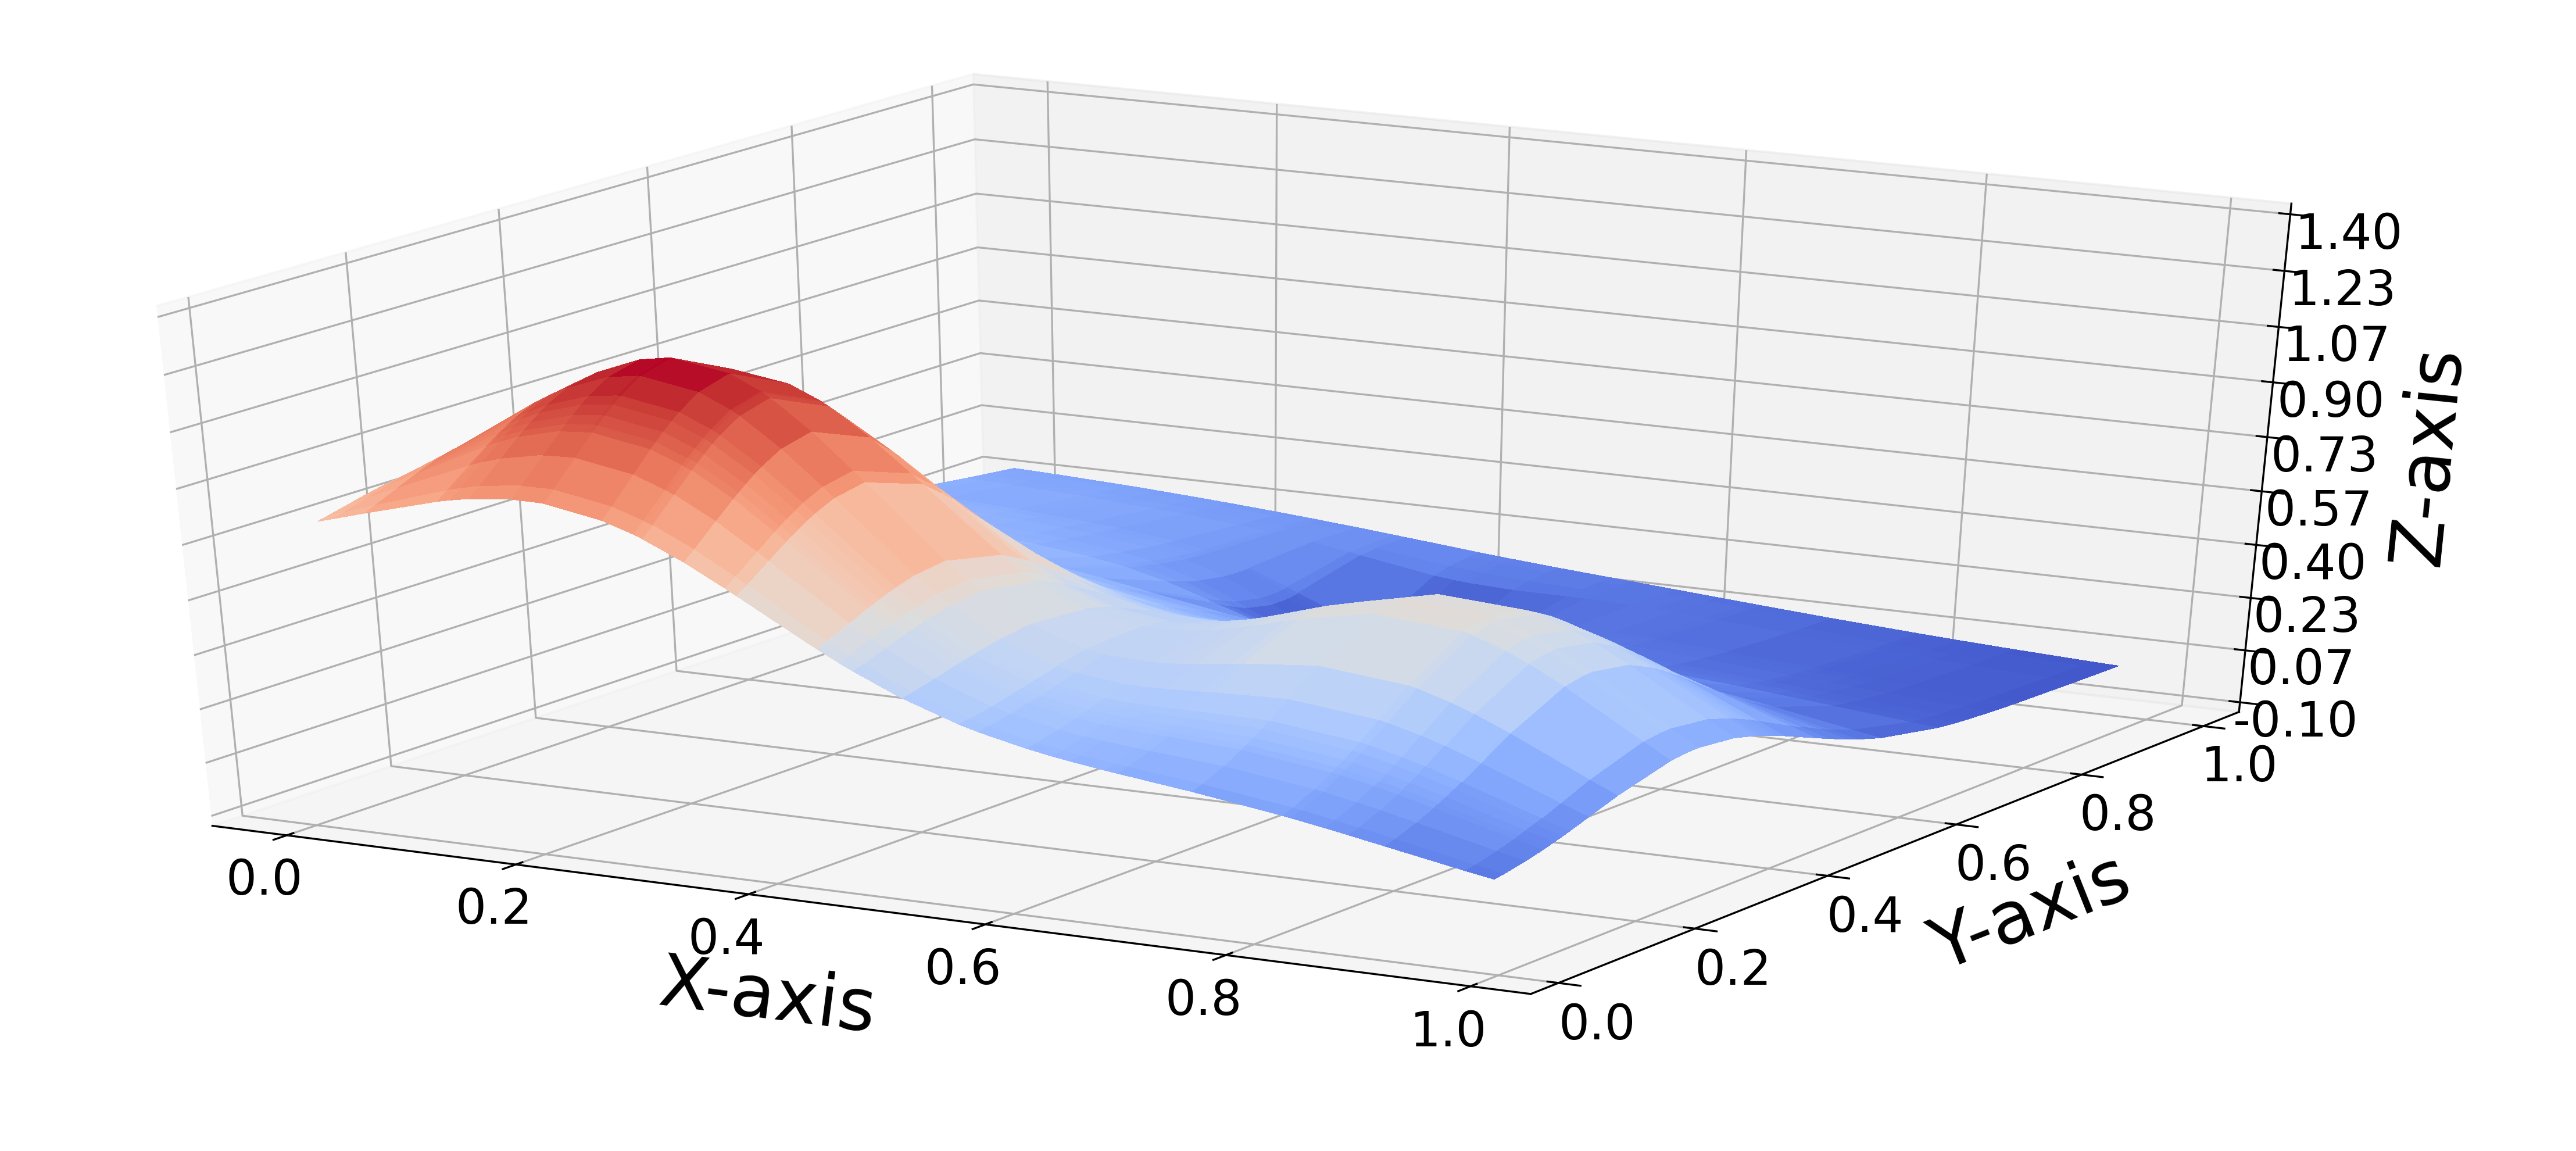
\includegraphics[width=7.9cm]{Figures/Franke_func.png}
\caption{Franke's function}
\label{fig:Frankplt}
\end{figure}

A last term  was added to Franke’s function (\ref{eq:Frank}) when generating data for the regression models. The new term contributed with a normal distributed noise $N(0,0.1)$.  


\subsubsection{MNIST data set}
This data set contains hand written digits from zero to nine.
The Tensorflow-Keras API \cite{chollet_keras_2015,martin_abadi_tensorflow_2015} was used to import 60.000 numbers in the training data set and 10.000 numbers in the test data set. Each hand written digit is a matrix where each number in the matrix represents the color in a gray scale image like in Figure \ref{fig:MNISTnumbers}.
\begin{figure}[!htb]
%\centering
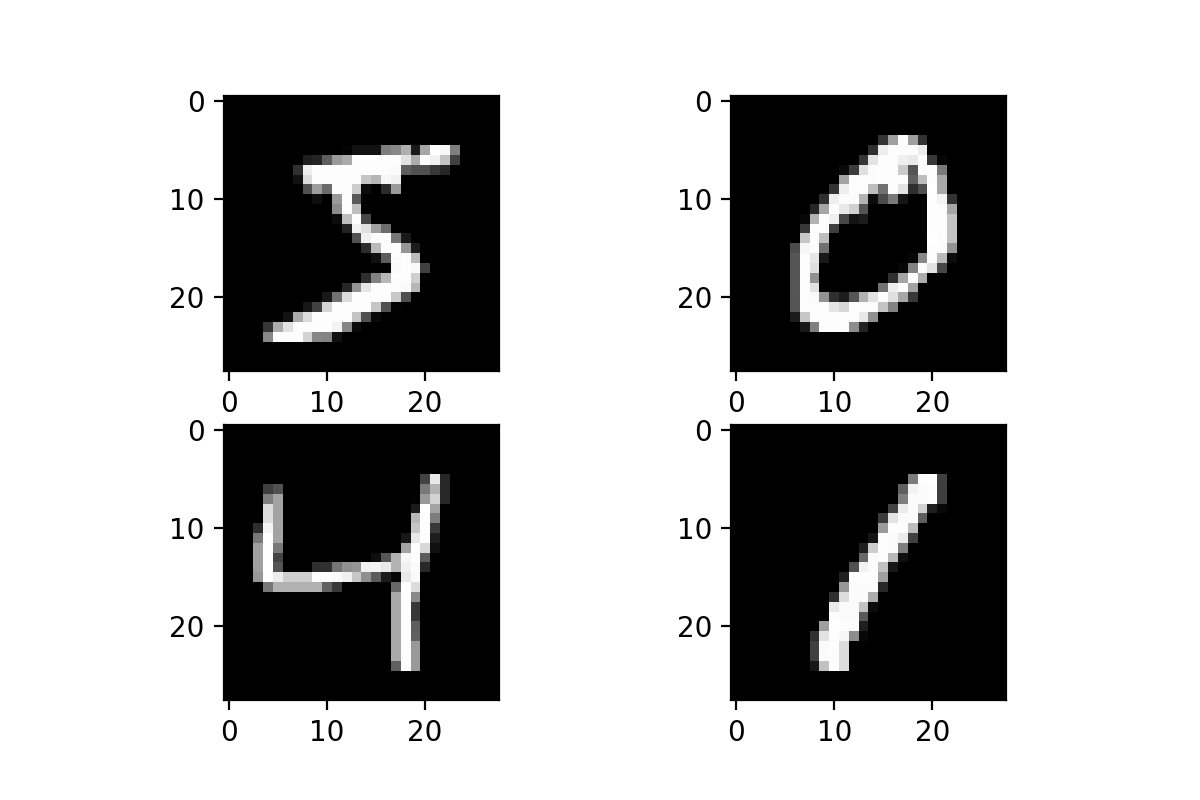
\includegraphics[width=7.9cm]{Figures/MNIST_number.png}
\caption{MNIST examples number}
\label{fig:MNISTnumbers}
\end{figure}
The image was flattened to a $784 x 1$ array which could be feed into the logistic regression and the Neural Network. The labels of each digit is a number between 0 and 9 and the distribution of the 10 different classes in the traing and test set can be seen in Figure \ref{fig:MNISTtrain} and Figure \ref{fig:MNISTtest}


\begin{figure}[!htbp]
%\centering
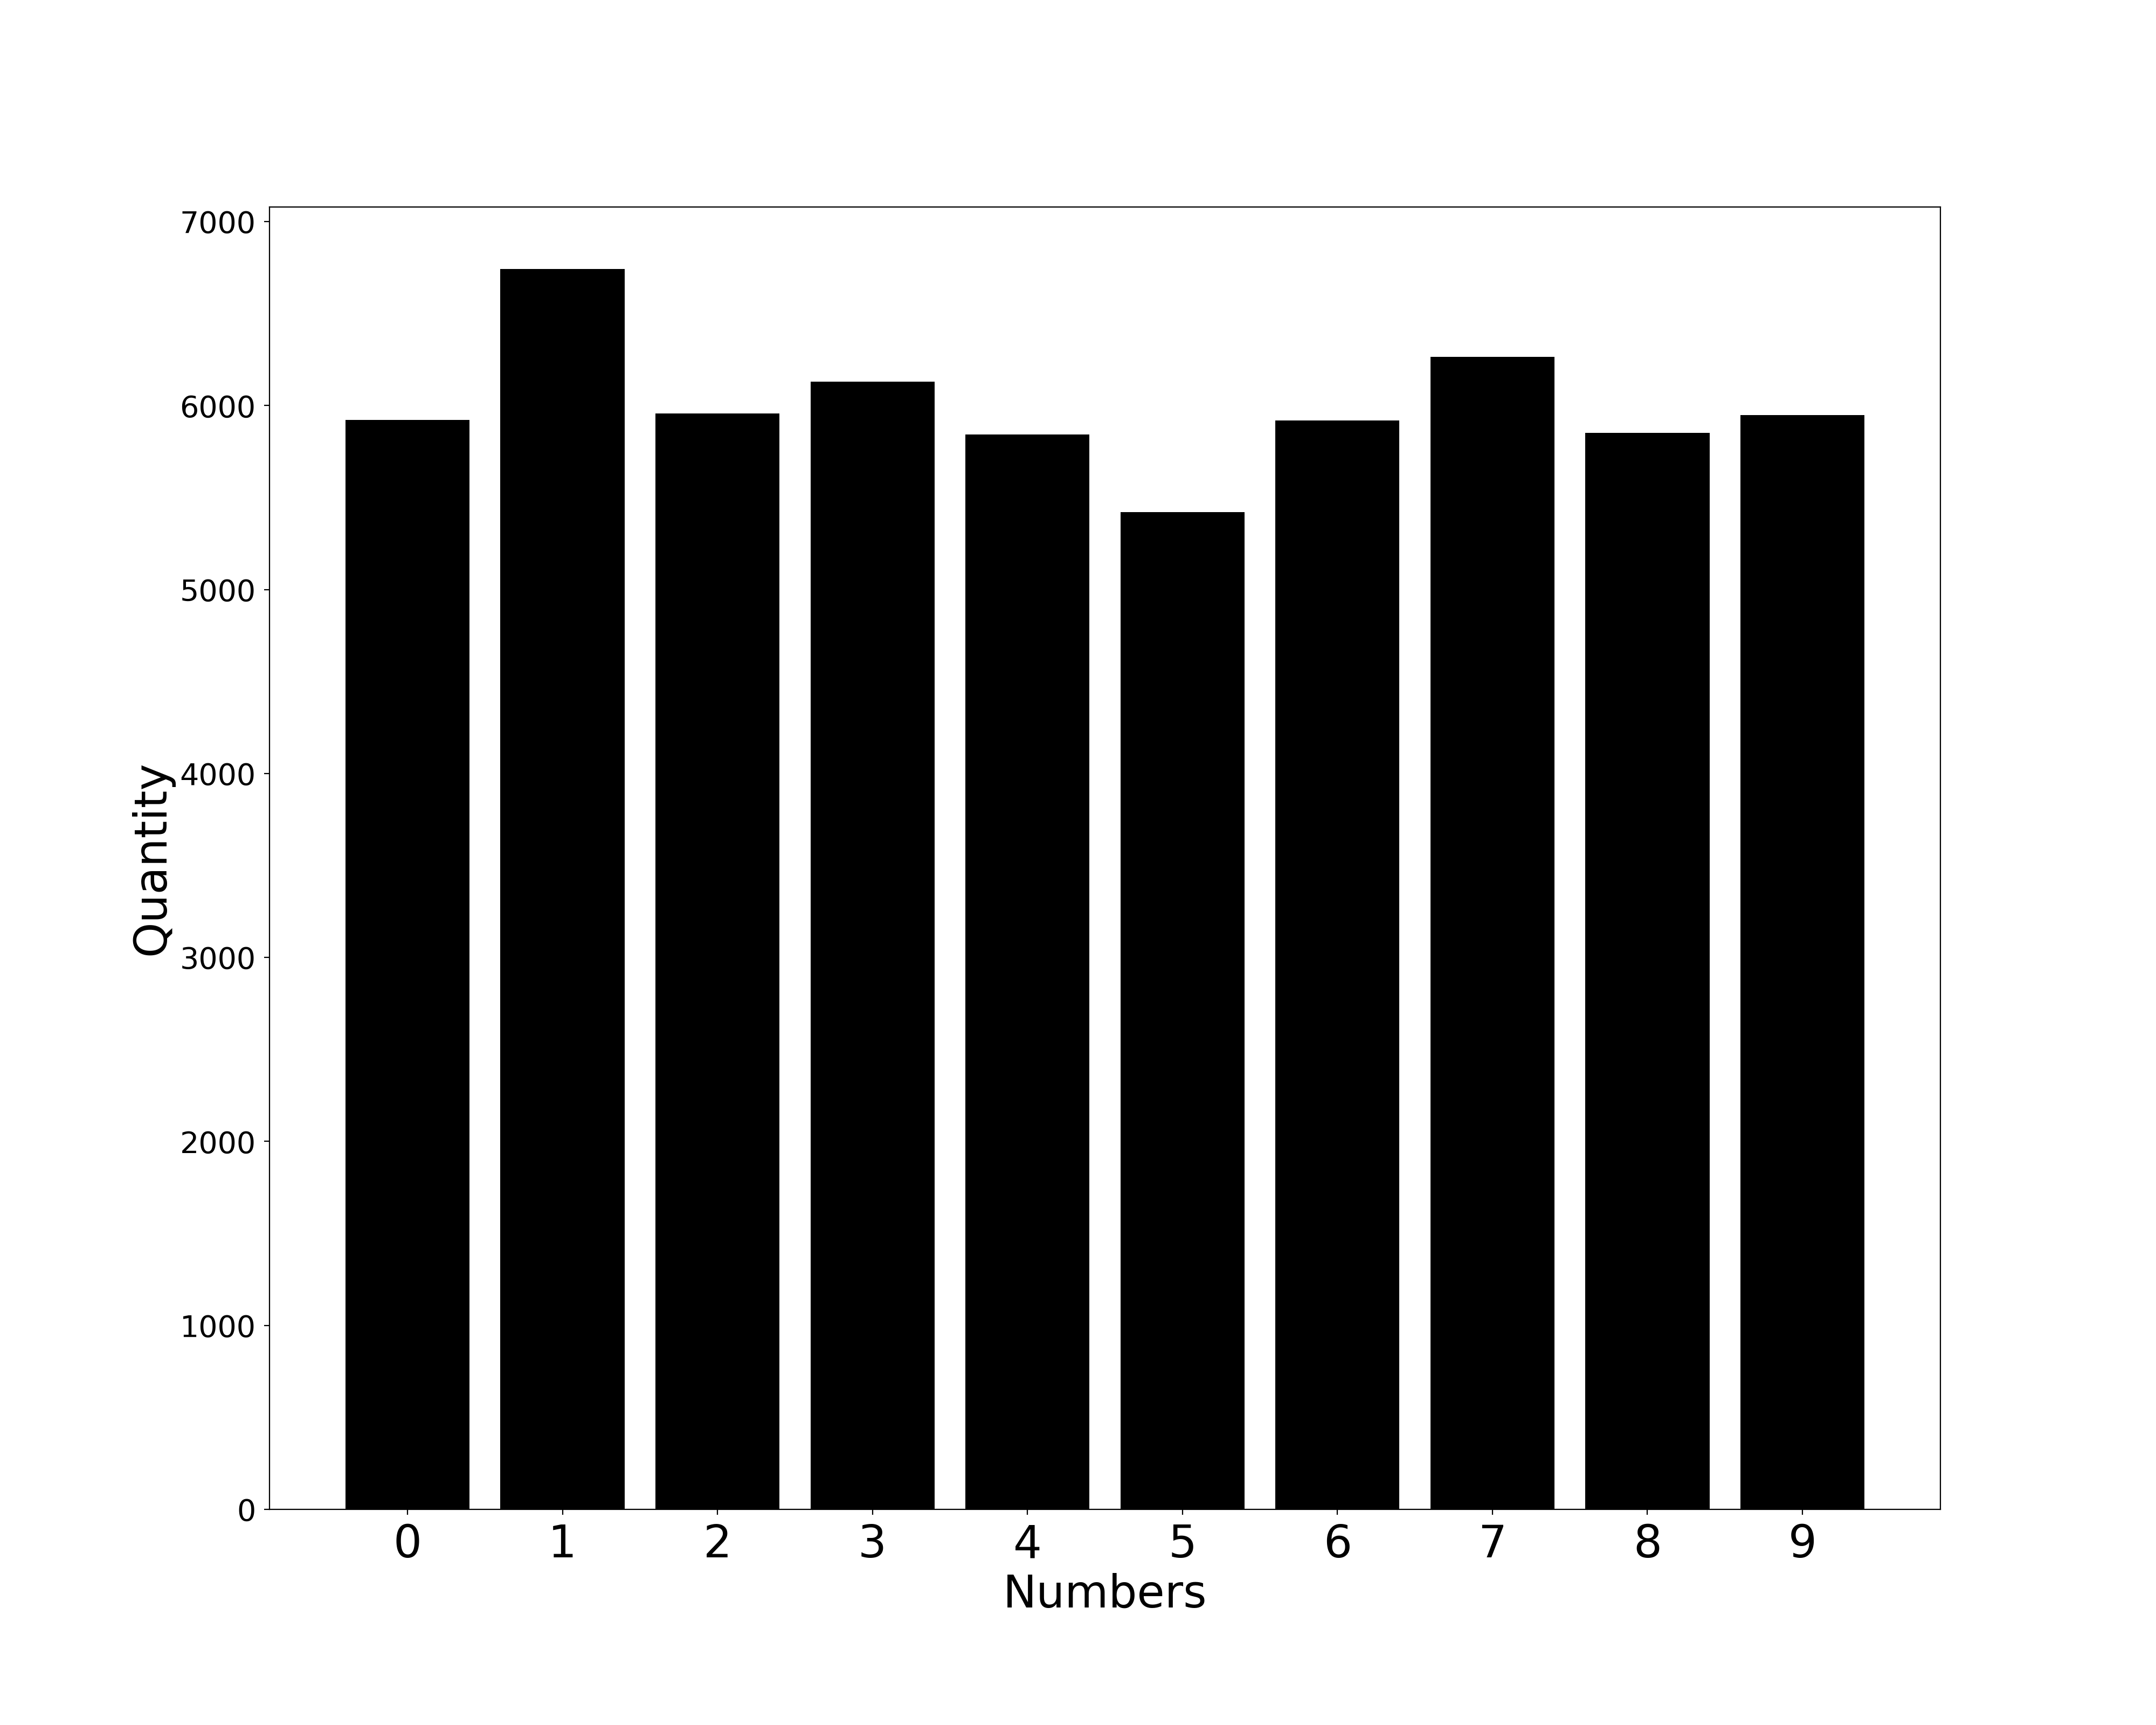
\includegraphics[width=7.9cm]{Figures/MNIST_train_data.png}
\caption{MNIST training data}
\label{fig:MNISTtrain}
\end{figure}


\begin{figure}[!htbp]
%\centering
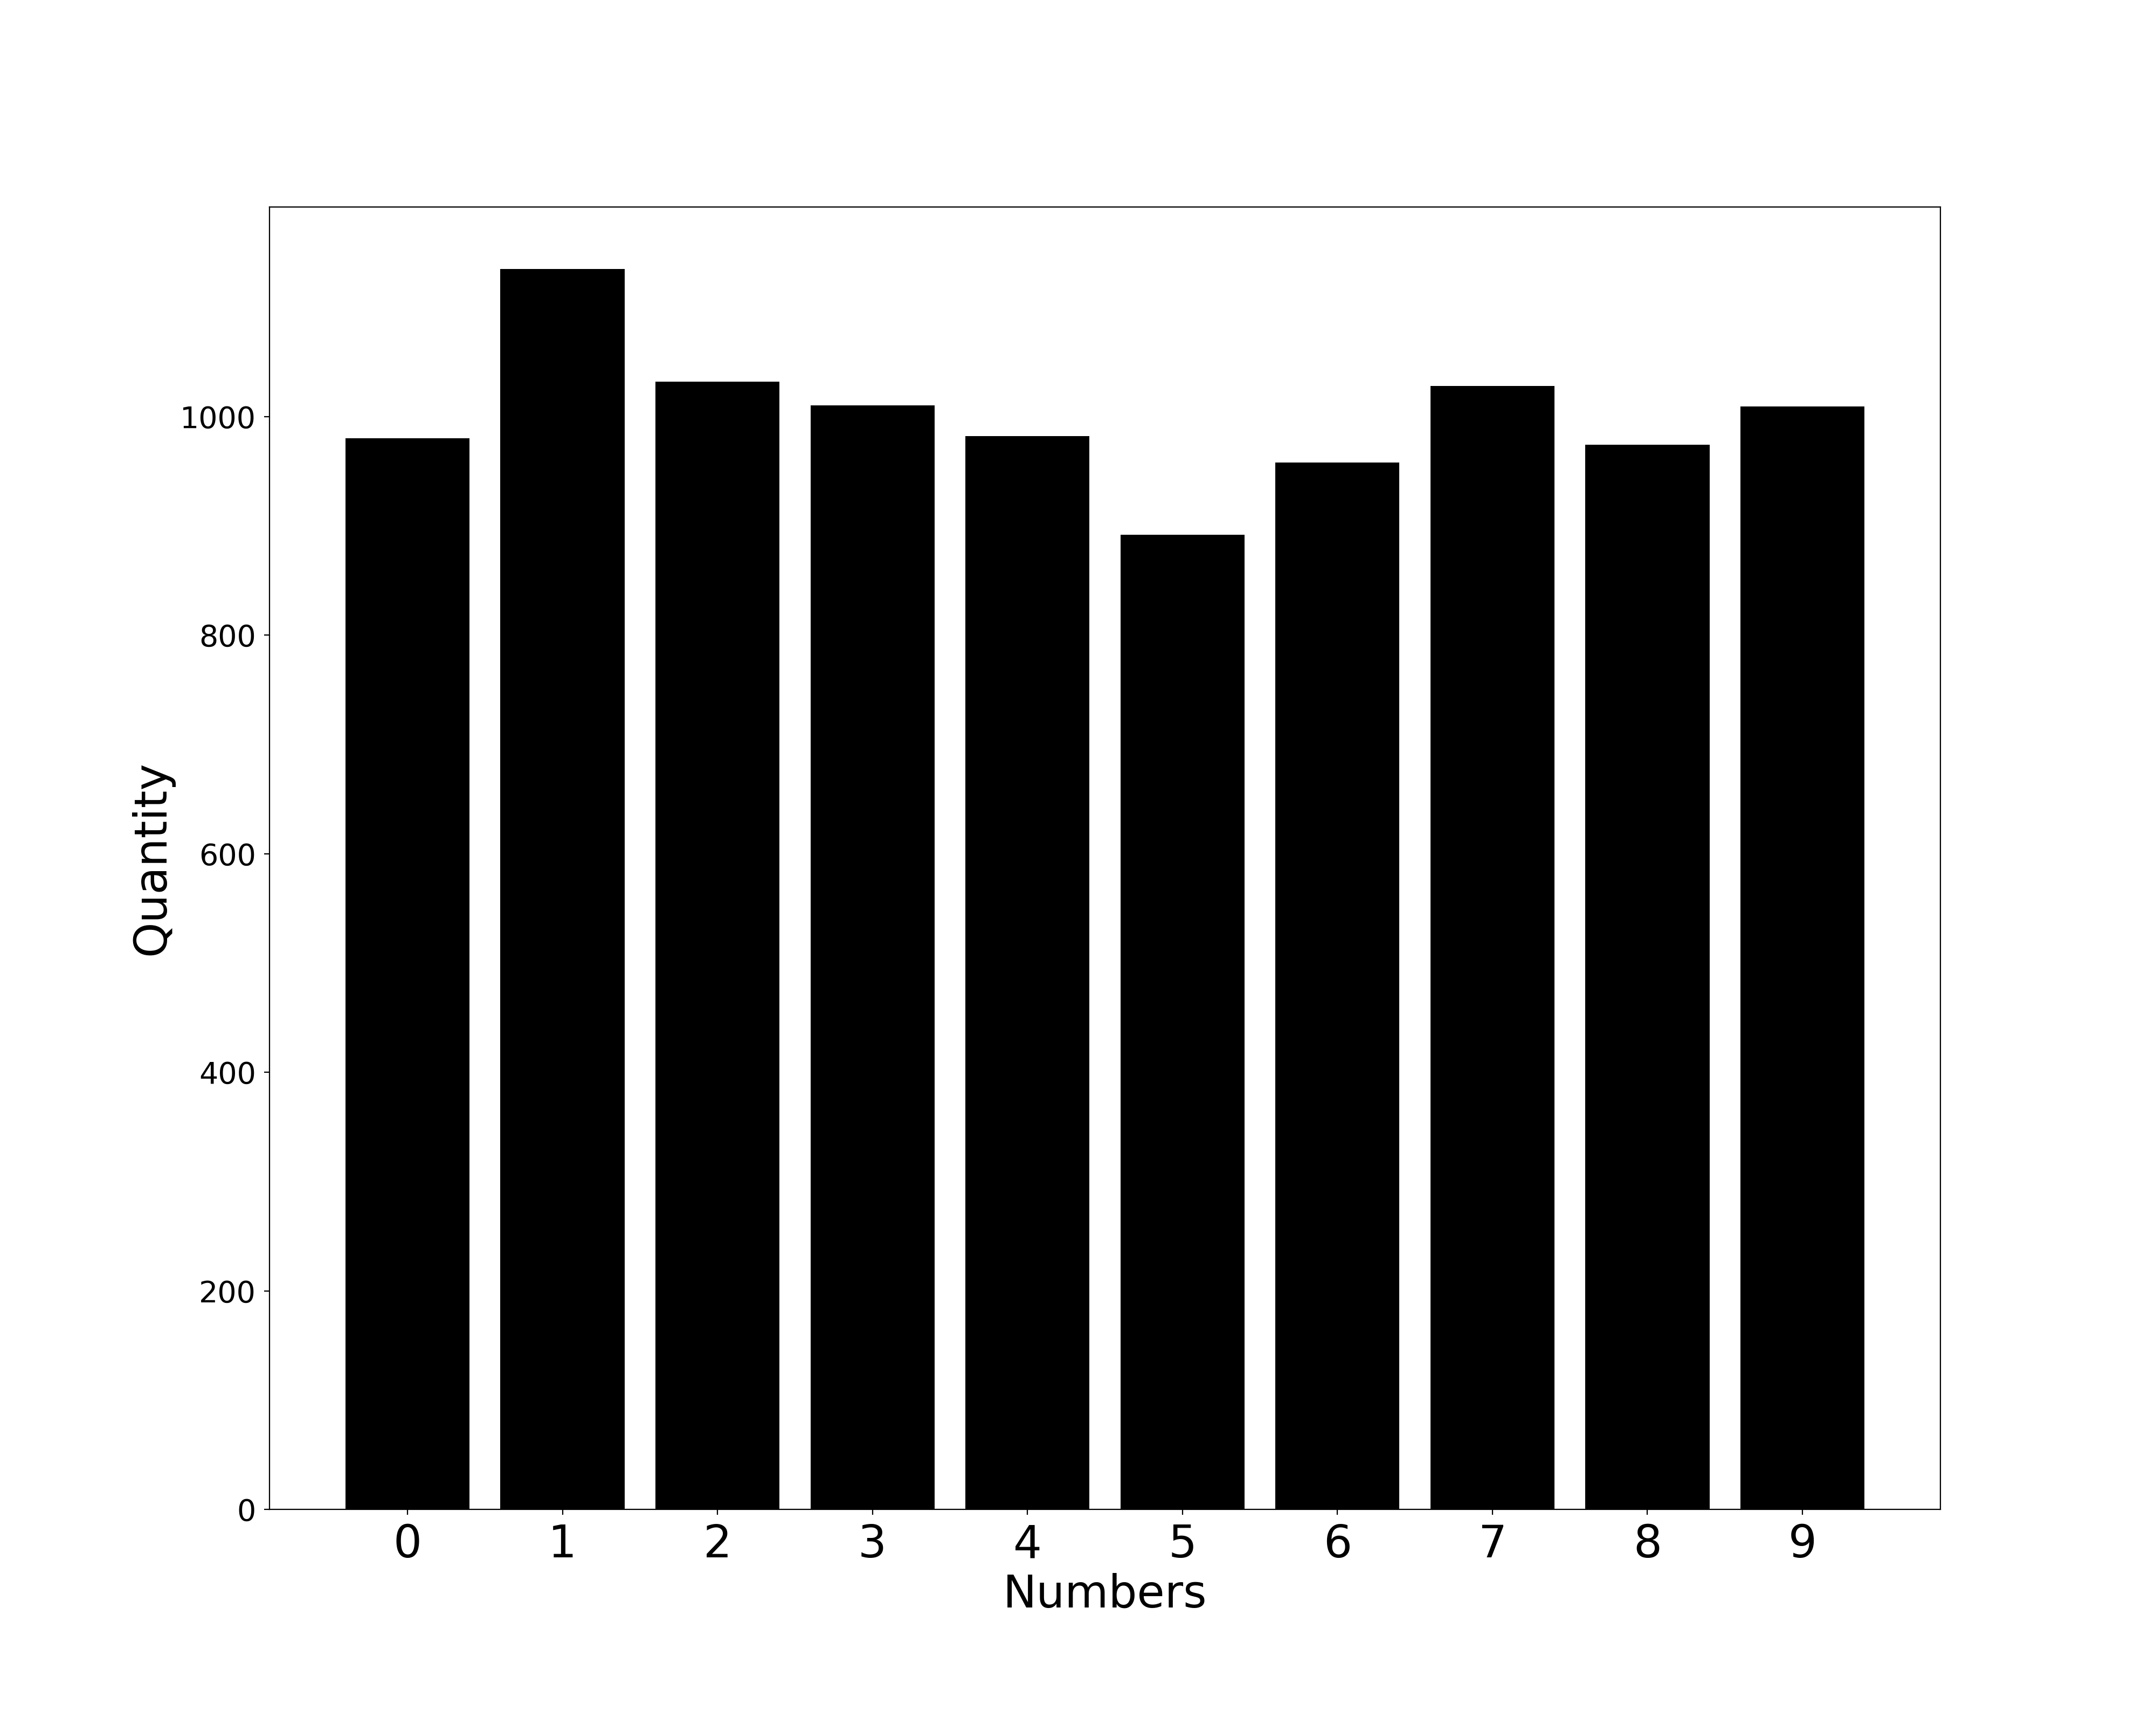
\includegraphics[width=7.9cm]{Figures/MNIST_test_data.png}
\caption{MNIST test data}
\label{fig:MNISTtest}
\end{figure}


\subsubsection{ECG-data}
The ECG data sets contained a total of 21837 12-lead ECGs from 18885 different patients. All recordings were 10 seconds long and each recording were available as a recording sampled at 500 Hz or down sampled to 100 Hz. In this study 500Hz was used. The labels of this data set was the diagnosis given by one or two cardiologists. There was 24 diagnoses present in the data set and they were categorized into five broader categories which are used in this study. A patient could be diagnosed into one or more of these five categories which makes this a multi-label, multi-class classification problem. The data set provider has proposed a test-training-split to make the results comparable across different studies \cite{wagner_ptb-xl_2020}. A stratified fold was used to give the same distribution of diagnoses in the train (see Figure \ref{fig:ECGtrain}) and test (see Figure \ref{fig:ECGtest}) set.

\begin{figure}[!htb]
%\centering
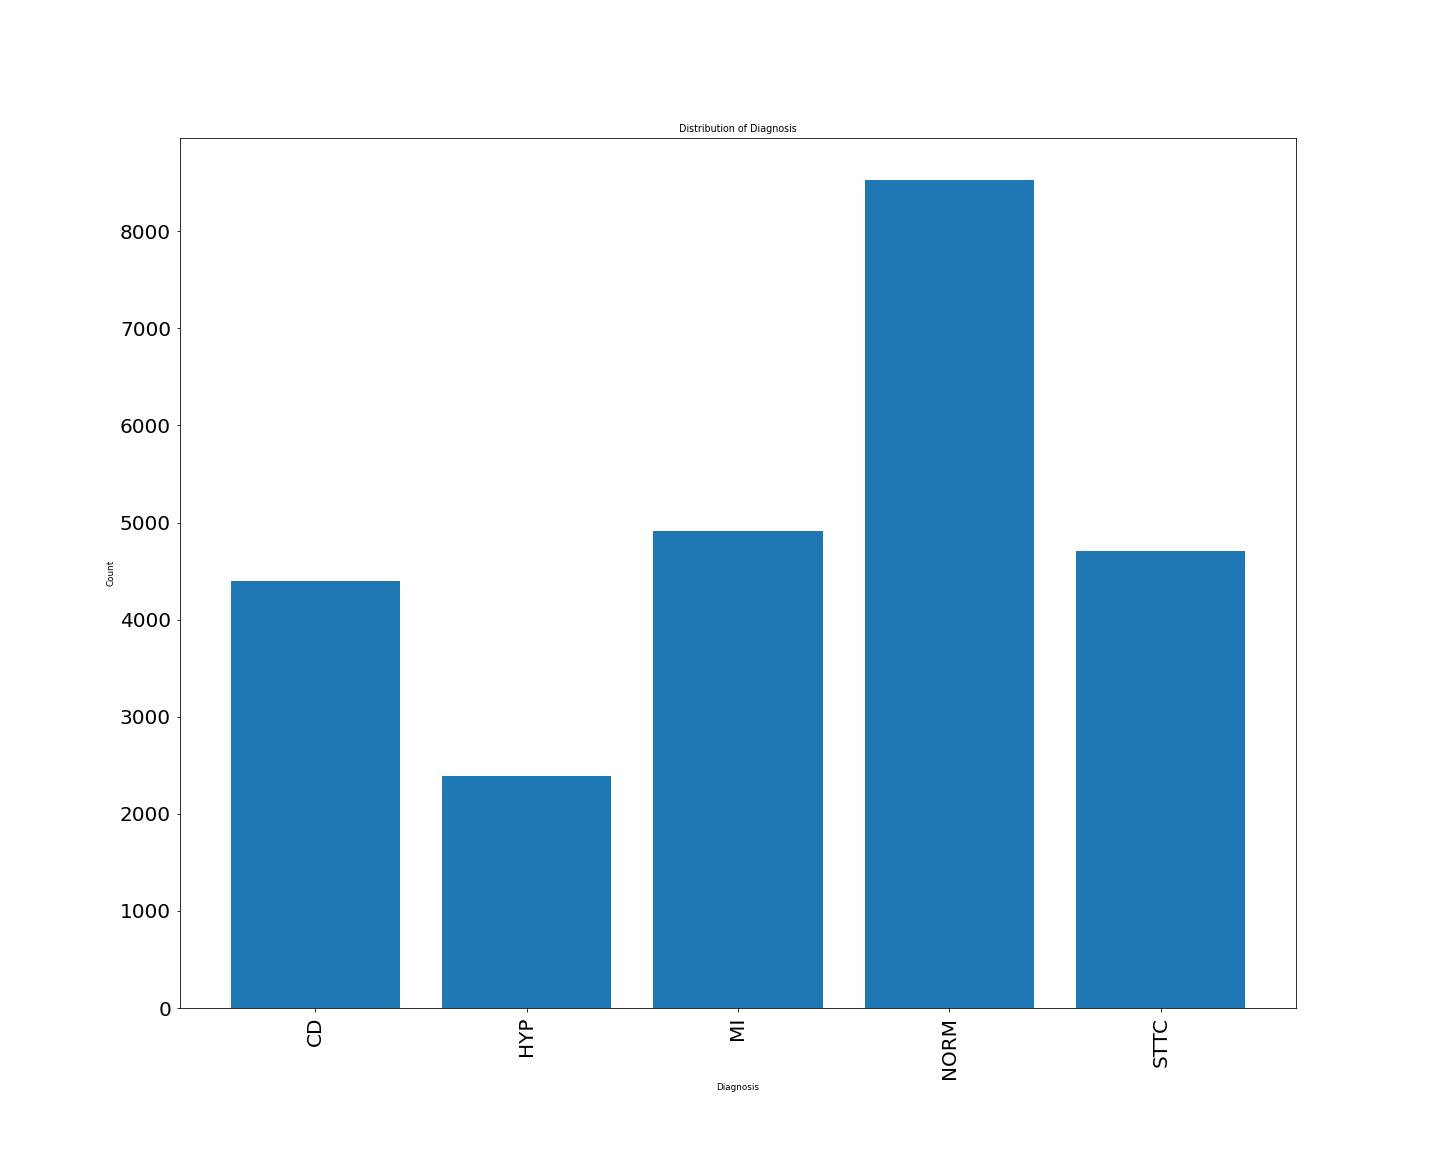
\includegraphics[width=7.9cm]{Figures/distribution_training.png}
\caption{ECG train data}
\label{fig:ECGtrain}
\end{figure}

\begin{figure}[!htb]
%\centering
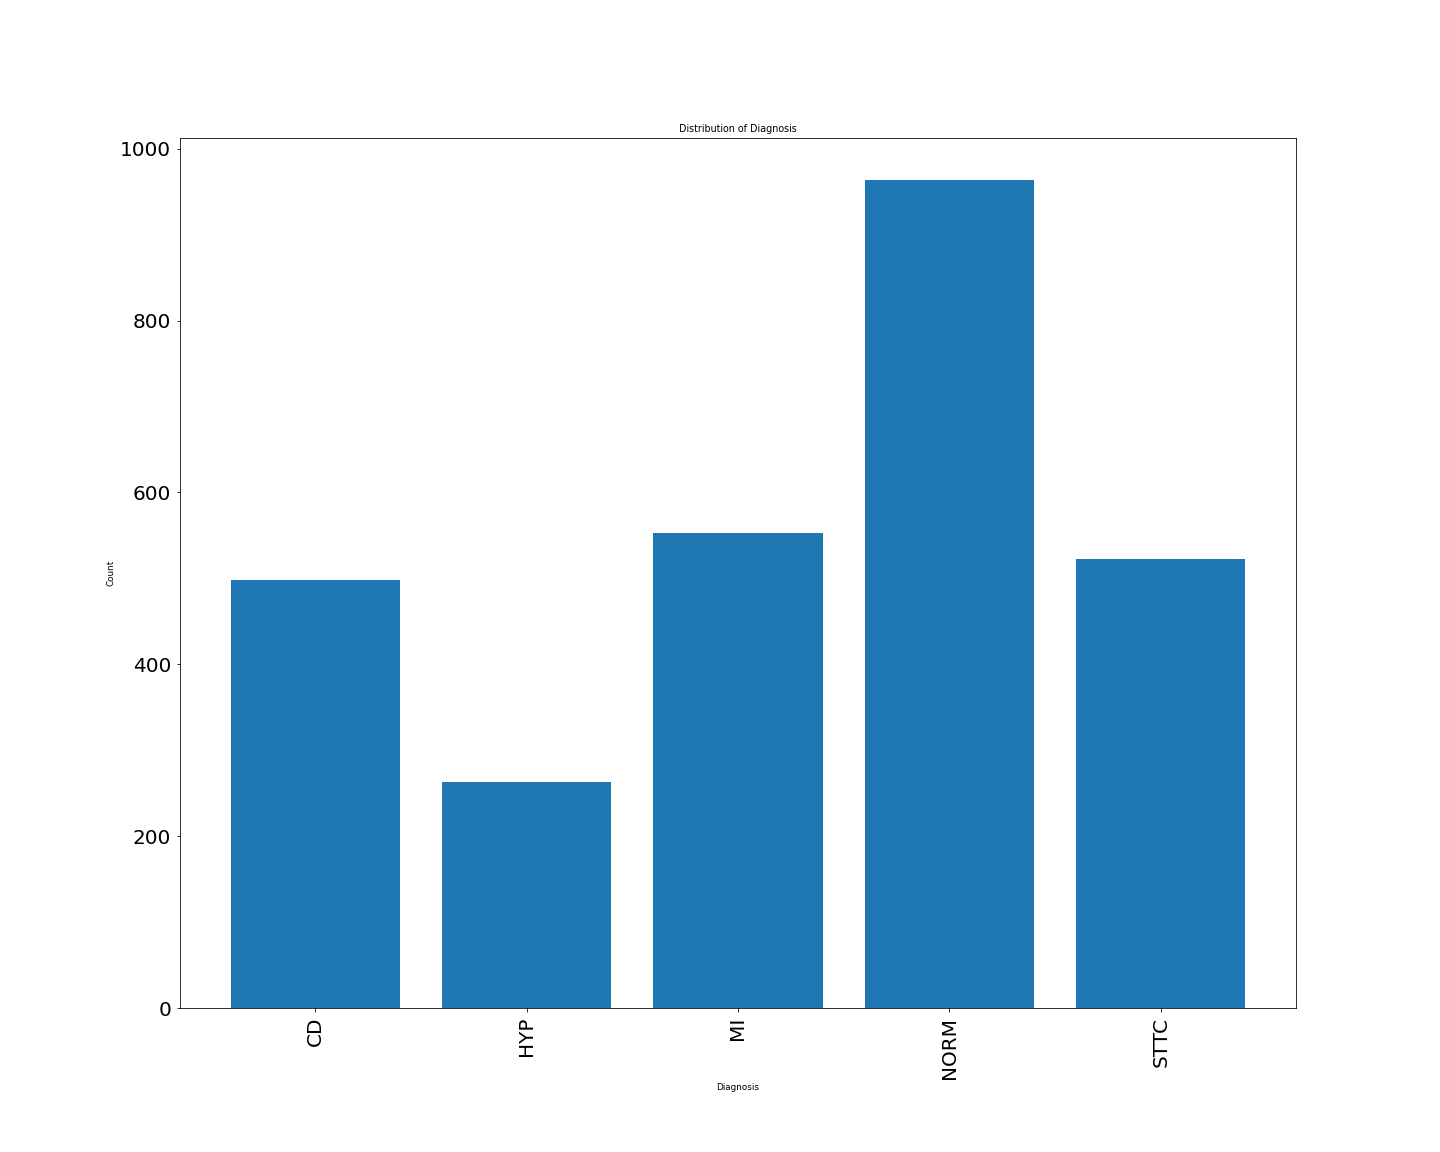
\includegraphics[width=7.9cm]{Figures/distribution_test.png}
\caption{ECG test data}
\label{fig:ECGtest}
\end{figure}

To be able to use the ECG data as input to a classifier, such as a Neural Network or a logistic regression model, the data was processed by extracting features instead of using the whole waveform as an input. This was done by developing a new Python package, ECG-featurizer\cite{bjorn-jostein_singstad_ecg-featurizer_nodate}, based on NeuroKit2 \cite{makowski_neurokit2_2020} and the Waveform database (WFDB) package. The ECG-featurizer extracted 112 features from each ECG-recording.


\subsection{Regression algorithms}
\subsubsection{Linear regression with SGD optimizer}
As a starting point for the regression analysis the OLS and Ridge regression models developed in \cite{bjorn-jostein_singstad_using_nodate} was trained once again. First, the polynomial degree of the OLS model was found using a search from polynomial degree one to 20 using the mean of a 10-fold cross validated R2-score.
The best polynomial degree from the OLS model were used as the degree in the Ridge model and a search through $\lambda$-values from $0.000001$ to $1000$ increasing with a factor of $10$ for each step. The best $\lambda$-values were selected based on the mean of a 10-fold cross validated R2-score.

Further, the design matrix in the OLS-algorithm were replaced with a stochastic gradient descent (SGD) optimization algorithm and employed on the data generated by Franke's function. A grid search was performed and a 3-fold cross validated accuracy score was used to find the optimal parameters of the learning rate ($\gamma)$, batch size, learning rate reduction and number of epochs.

\subsubsection{Regression using Neural Network}
A Neural Network with linear activation in the final layer was developed. The linear activation in the final layer was necessary for the purpose of doing regression. The optimal parameters were found doing two grid search. The first grid search were serching for the optimal learning rate, number of hidden layers, number of hidden units (neurons), activation functions in the hidden layer. The second grid search were searching for the optimal number of epochs, batch size, weight initialization, and bias initialization. The optimal parameters found in grid search one were used in grid search two. 3-fold cross validation was used during both grid search and the best mean R2-score over the three folds were used as the measure for selecting parameters.

\subsection{Classification}
\subsubsection{Classifying MNIST data}

The neural network used to classify MNIST data used Softmax activation (eq \ref{eq:softmax})in the final layer. This is typical for a classification problem were each input data only have one label (not multi-label).
\begin{equation}
softmax(x)_i = \frac{exp(x_i)}{\sum_{j}^{ }exp(x_j))}
\label{eq:softmax}
\end{equation}
The optimal parameters of the Neural Network were found using graduate student descent method. The model with the optimal parameters were validated using 5-fold cross validation and tested on a unused test set.

In addition a Logistic Regression algorithm was developed, tested and compared with the Neural Network.

\subsubsection{Classifying PTB-XL ECG data}
Since the PTB-XL ECG data were a multi-class, multi-label classification problem the Neural Network had to use a Sigmoid activation(eq \ref{eq:sigmoid}) in the final layer
\begin{equation}
h_ \theta (x) =  \frac{\mathrm{1} }{\mathrm{1} + e^-\theta^Tx}
    \label{eq:sigmoid}
\end{equation}
The hyper parameters were optimized using Bayesian Tuner \cite{omalley_keras_2019}. The 1st validation fold of a 10-fold stratified cross validation was used for the optimization to speed up the search. 

The ECG classification and thus the prediction threshold had to be set. The threshold  were optimized when the model was successfully trained . This was done by running the classifier on the test set  and receiving a score between 0 and 1 for each of the classes. A search trough thresholds were done using a 5-bit long array of ones and that got multiplied with values from 0 to 1 with a step size of 0.01 which resulted in 100 different threshold. The accuracy score for the training data were evaluated for each threshold. The best threshold were used as a initial guess for the Nelder-Mead downhill simplex method \cite{nelder_simplex_1965, virtanen_scipy_2020}. This algorithm optimized the threshold for each class individually. The Nelder-Mead downhill simplex method is used to find the local minimum of a function using the function itself and an initial guess of the variable of the function. The 5-element long array was optimized using the negative of the accuracy score and thus resulted in the best possible accuracy score for the given model.

Also a a Logistic Regression algorithm was developed, tested and compared with the Neural Network.


\section{Results}
\subsection{Regression}
\subsubsection{OLS}
The best polynomial degree of the OLS algorithm based on the mean of a 10-fold cross validated R2-score. Polynomial degrees from 1 to 20 were tested and a degree of 9 turned out to be best.
\subsubsection{Ridge}
The polynomial degree of 9 were used in the Ridge model and $\labdas$ from $0.000001$ to $1000$ were tested and selected using the mean of a 10-fold cross validated R2-score. The best $\labdas$ turned out to be $0.1$

Both the OLS and the Ridge model were then cross validated using their optimized parameter. The cross validated R2-score for OLS was: median$=0.831 \pm0.019$SD and median$=0.015 \pm0.002$SD for MSE. The cross validated R2-score for Ridge was: median$=0.830 \pm0.016$SD.\newline
MSE Ridge:$=0.015 \pm0.001$SD for MSE. The results are also presented in figure \ref{fig:OLS_ridge}.
\begin{figure}[htbp!]
%\centering
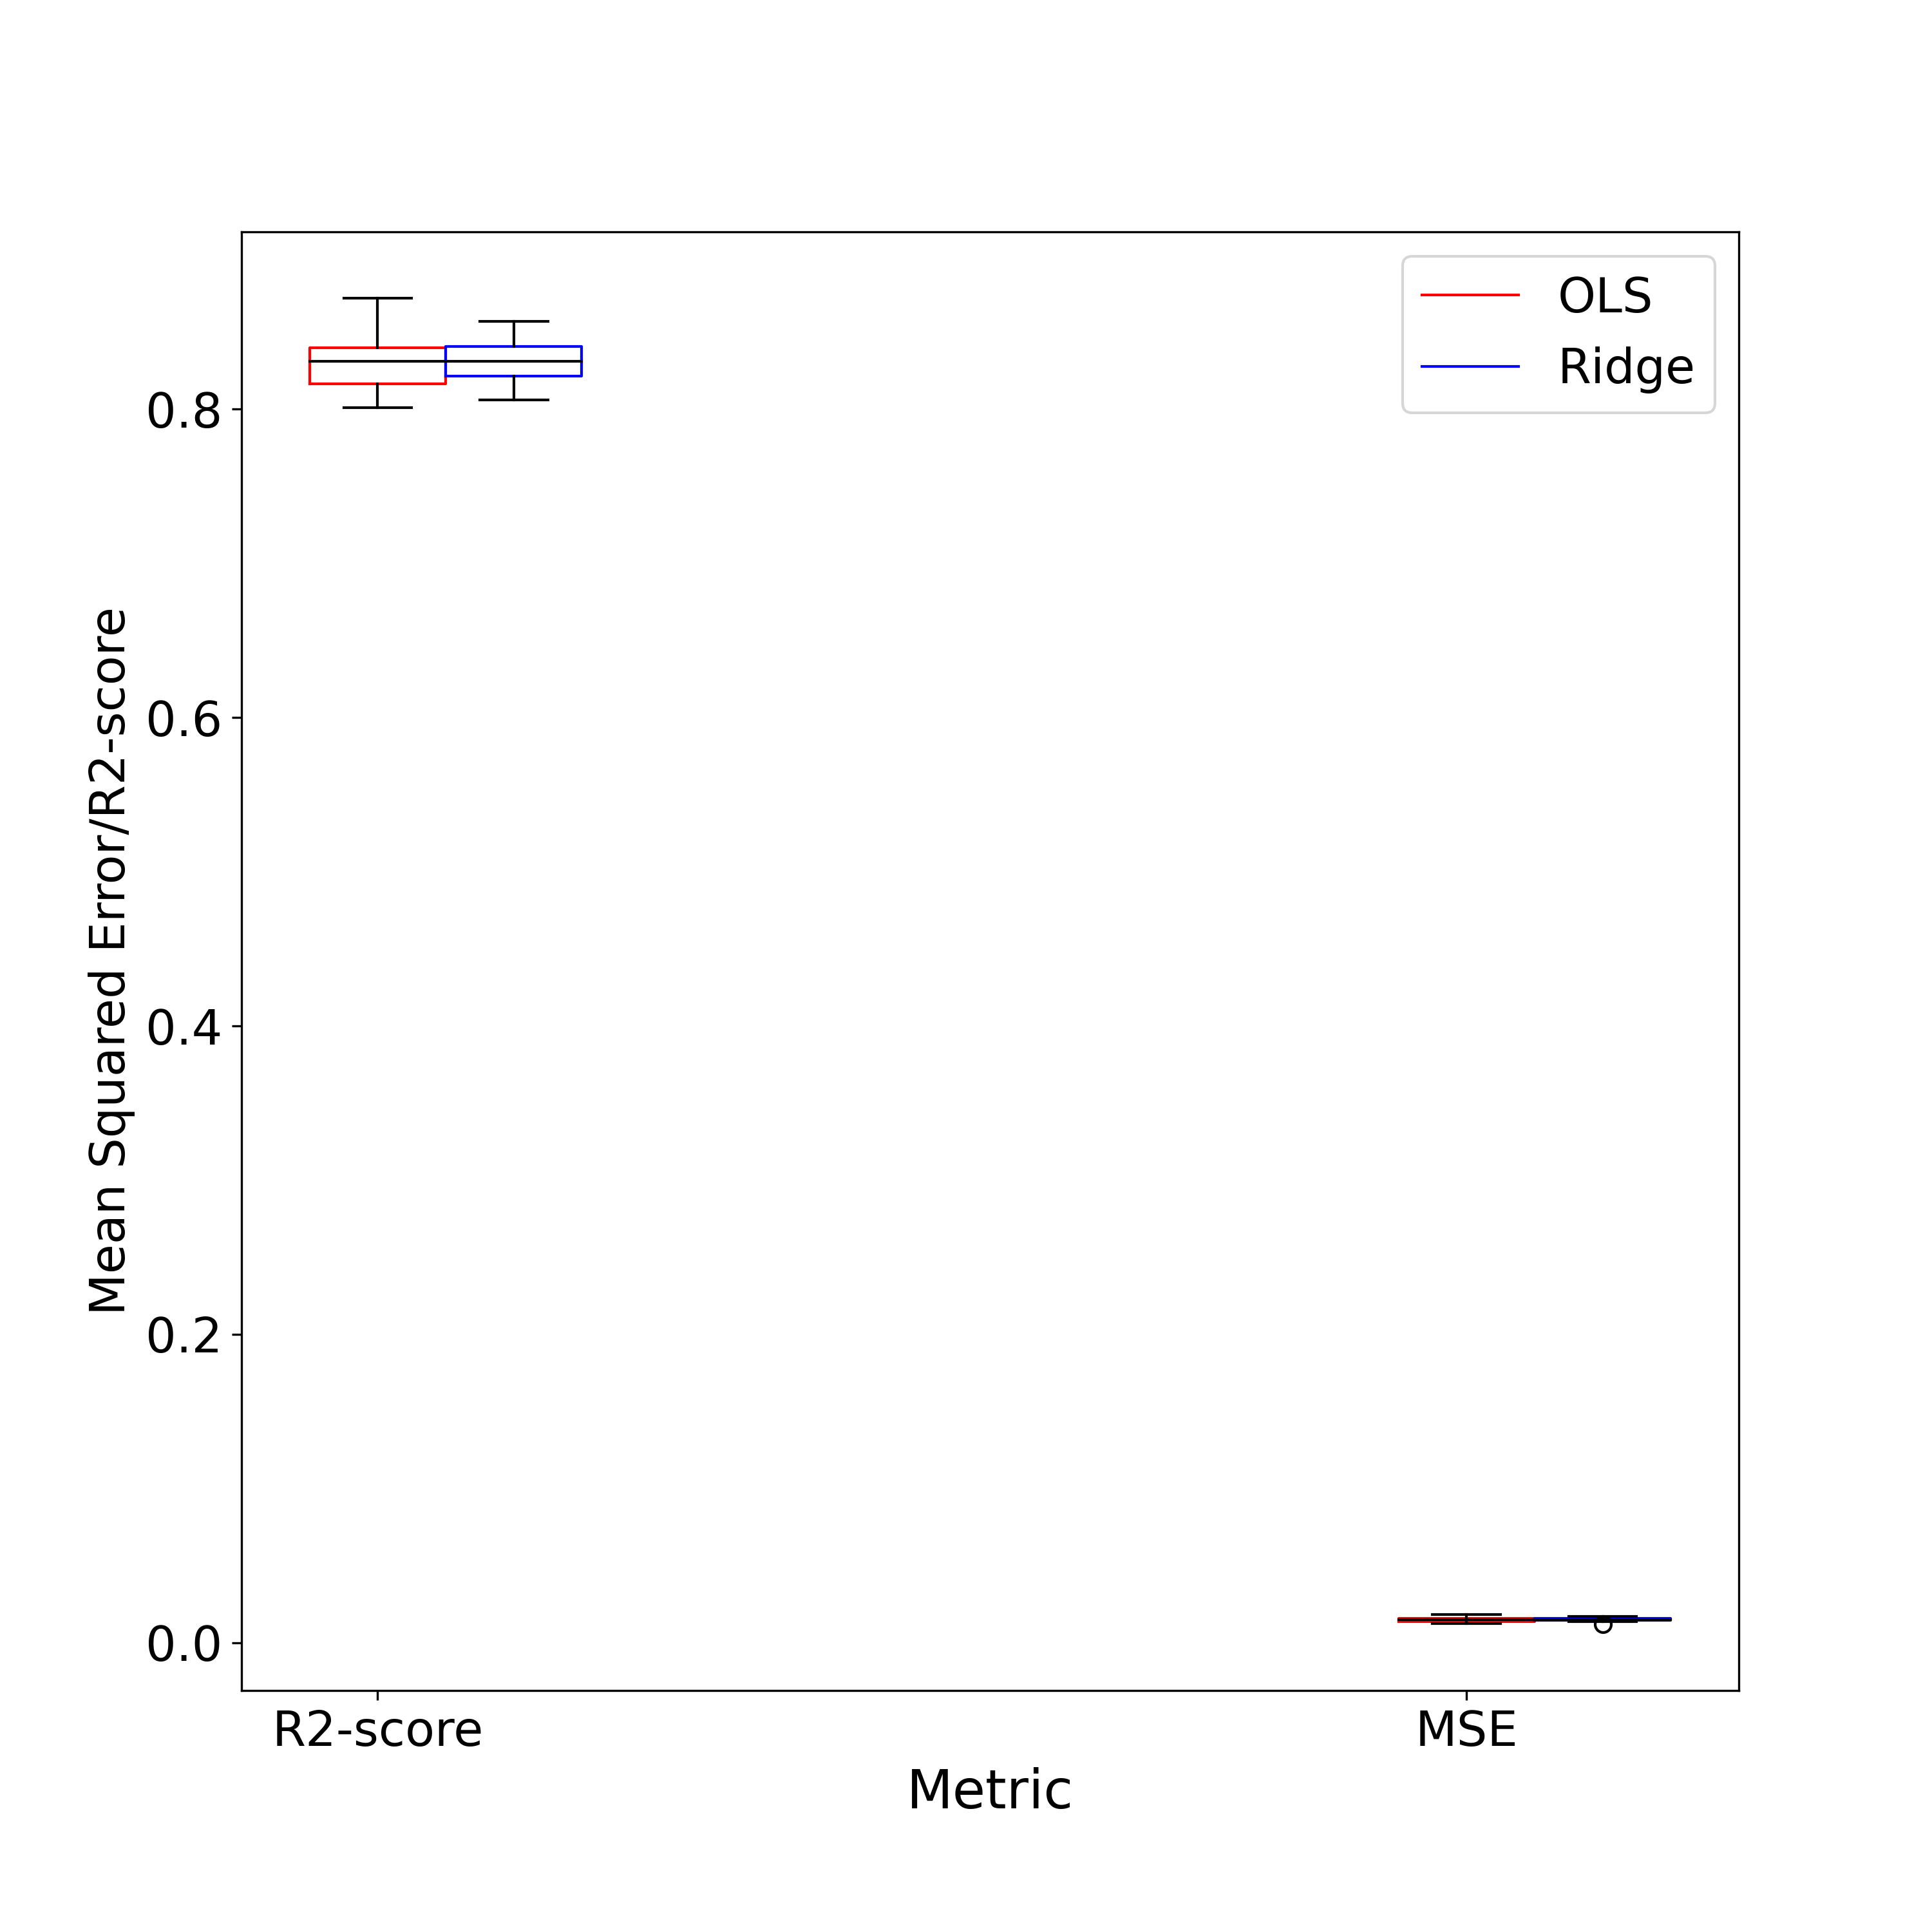
\includegraphics[width=7.9cm]{Figures/boxplot_OLS_ridge.png}
\caption{The red boxes shows the cross validated R2-score and MSE achieved by the OLS algorithm using a polynomial degree$=9$. The blue boxes shows the cross validated R2-score and MSE achieved by the Ridge algorithm using a polynomial degree$=9$ and a $\lambda = 0.1$}
\label{fig:OLS_ridge}
\end{figure}

\subsubsection{SGD OLS}
The SGD OLS model selection were done using 3 fold cross validation. The parameters that were search through using grid search were: 

\vspace{-4 mm}
\begin{table}[!htpb]
\vspace{4 mm}
\caption{\label{tab:gridsearch_sgd} Grid search parameters used to optimize OLS SGD}
\centerline{\begin{tabular}{lr} \hline\hline
Parameter                       & Values         \\ \hline
Learning rate ($\gamma$   &  $0.01, 0.001, 0.0001$  \\
Batch size             & $30,50,70$               \\ 
Learning rate reduction          & $10^{-5}, 10^{-3}, 10^{-1}$                \\  
Epochs & $5,10,15$ \\\hline\hline
\end{tabular}}

\end{table}

The results did not seem to be right and figure \ref{fig:appendix_sdg} shows the OLS SDG together with Ridge and OLS.


\subsubsection{Neural Network Regression}
Hyper parameters for the Neural network was found doing grid search on a small subset of the data generated by Frankes function. The resampling function from Scikit-learn \cite{pedregosa_scikit-learn_2011} was used to pick $200$ random samples from the total $1600$ data points. The parameter optimization were divided into two grid searches. The 1st grid search was done using the parameters in table \ref{tab:gridsearch_nn_reg}.


\vspace{-4 mm}
\begin{table}[!htpb]
\vspace{4 mm}
\caption{\label{tab:gridsearch_nn_reg} The parameters which were optimized using grid search on the Neural Network employed on a subset of Franke's function. Grid search nr1}

\centerline{\begin{tabular}{lr} \hline\hline
Parameter                       & Values                                \\ \hline
Learning rate                   &  $0.1,0.001,0.00001$                  \\                      
Hidden layers                   & $1,4,7$                               \\
Hidden units                    &  $50,100,150$                         \\
Activation in hidden layers     & ReLU, Sigmoid, SeLU                   \\\hline\hline
\end{tabular}}
\end{table}
The best parameters found in grid search 1 was then used in grid search 2. The parameters optimized in grid search 2 is shown in table \ref{tab:gridsearch_nn_reg2}.
\vspace{-4 mm}
\begin{table}[!htpb]
\vspace{4 mm}
\caption{\label{tab:gridsearch_nn_reg2} The parameters which were optimized using grid search on the Neural Network employed on a subset of Franke's function. Grid search nr 2}

\centerline{\begin{tabular}{lr} \hline\hline
Parameter                       & Values    \\ \hline
Epoch                   &  $10,50,100$  \\
Batch size                      & $10,50,100$     \\              
Bias initialization                   &  zeros, RandomNormal, RandomUniform     \\
Weight initialization                    & zeros, RandomNormal, RandomUniform   \\\hline\hline
\end{tabular}}
\end{table}

A 3-fold cross validation was used during grid search and the best mean of the R2-score computed for each fold were used as the measure for selecting the best parameters. 

Finally, the optimized parameters was used in the model when performing a 10-fold cross validation on the whole data set. The Neural Network achieved a cross validated R2-score of  median$=0.857\pm 0.021SD$ and a cross validated MSE of median$=0.012\pm 0.001SD$ 


\subsection{Neural Network classification}
\subsubsection{Classification of MNIST-data using Neural Network}
The optimal parameters of the neural network used to classify the MNIST data were found using graduate student descent. The model was then validated 5-fold cross validation and achieved a R2-score of: median=$0.851 \pm 0.002SD$. A confusion matrix for the model can be seen in figure \ref{fig:NN_mnist_confmatrix}.

\begin{figure}[htbp!]
%\centering
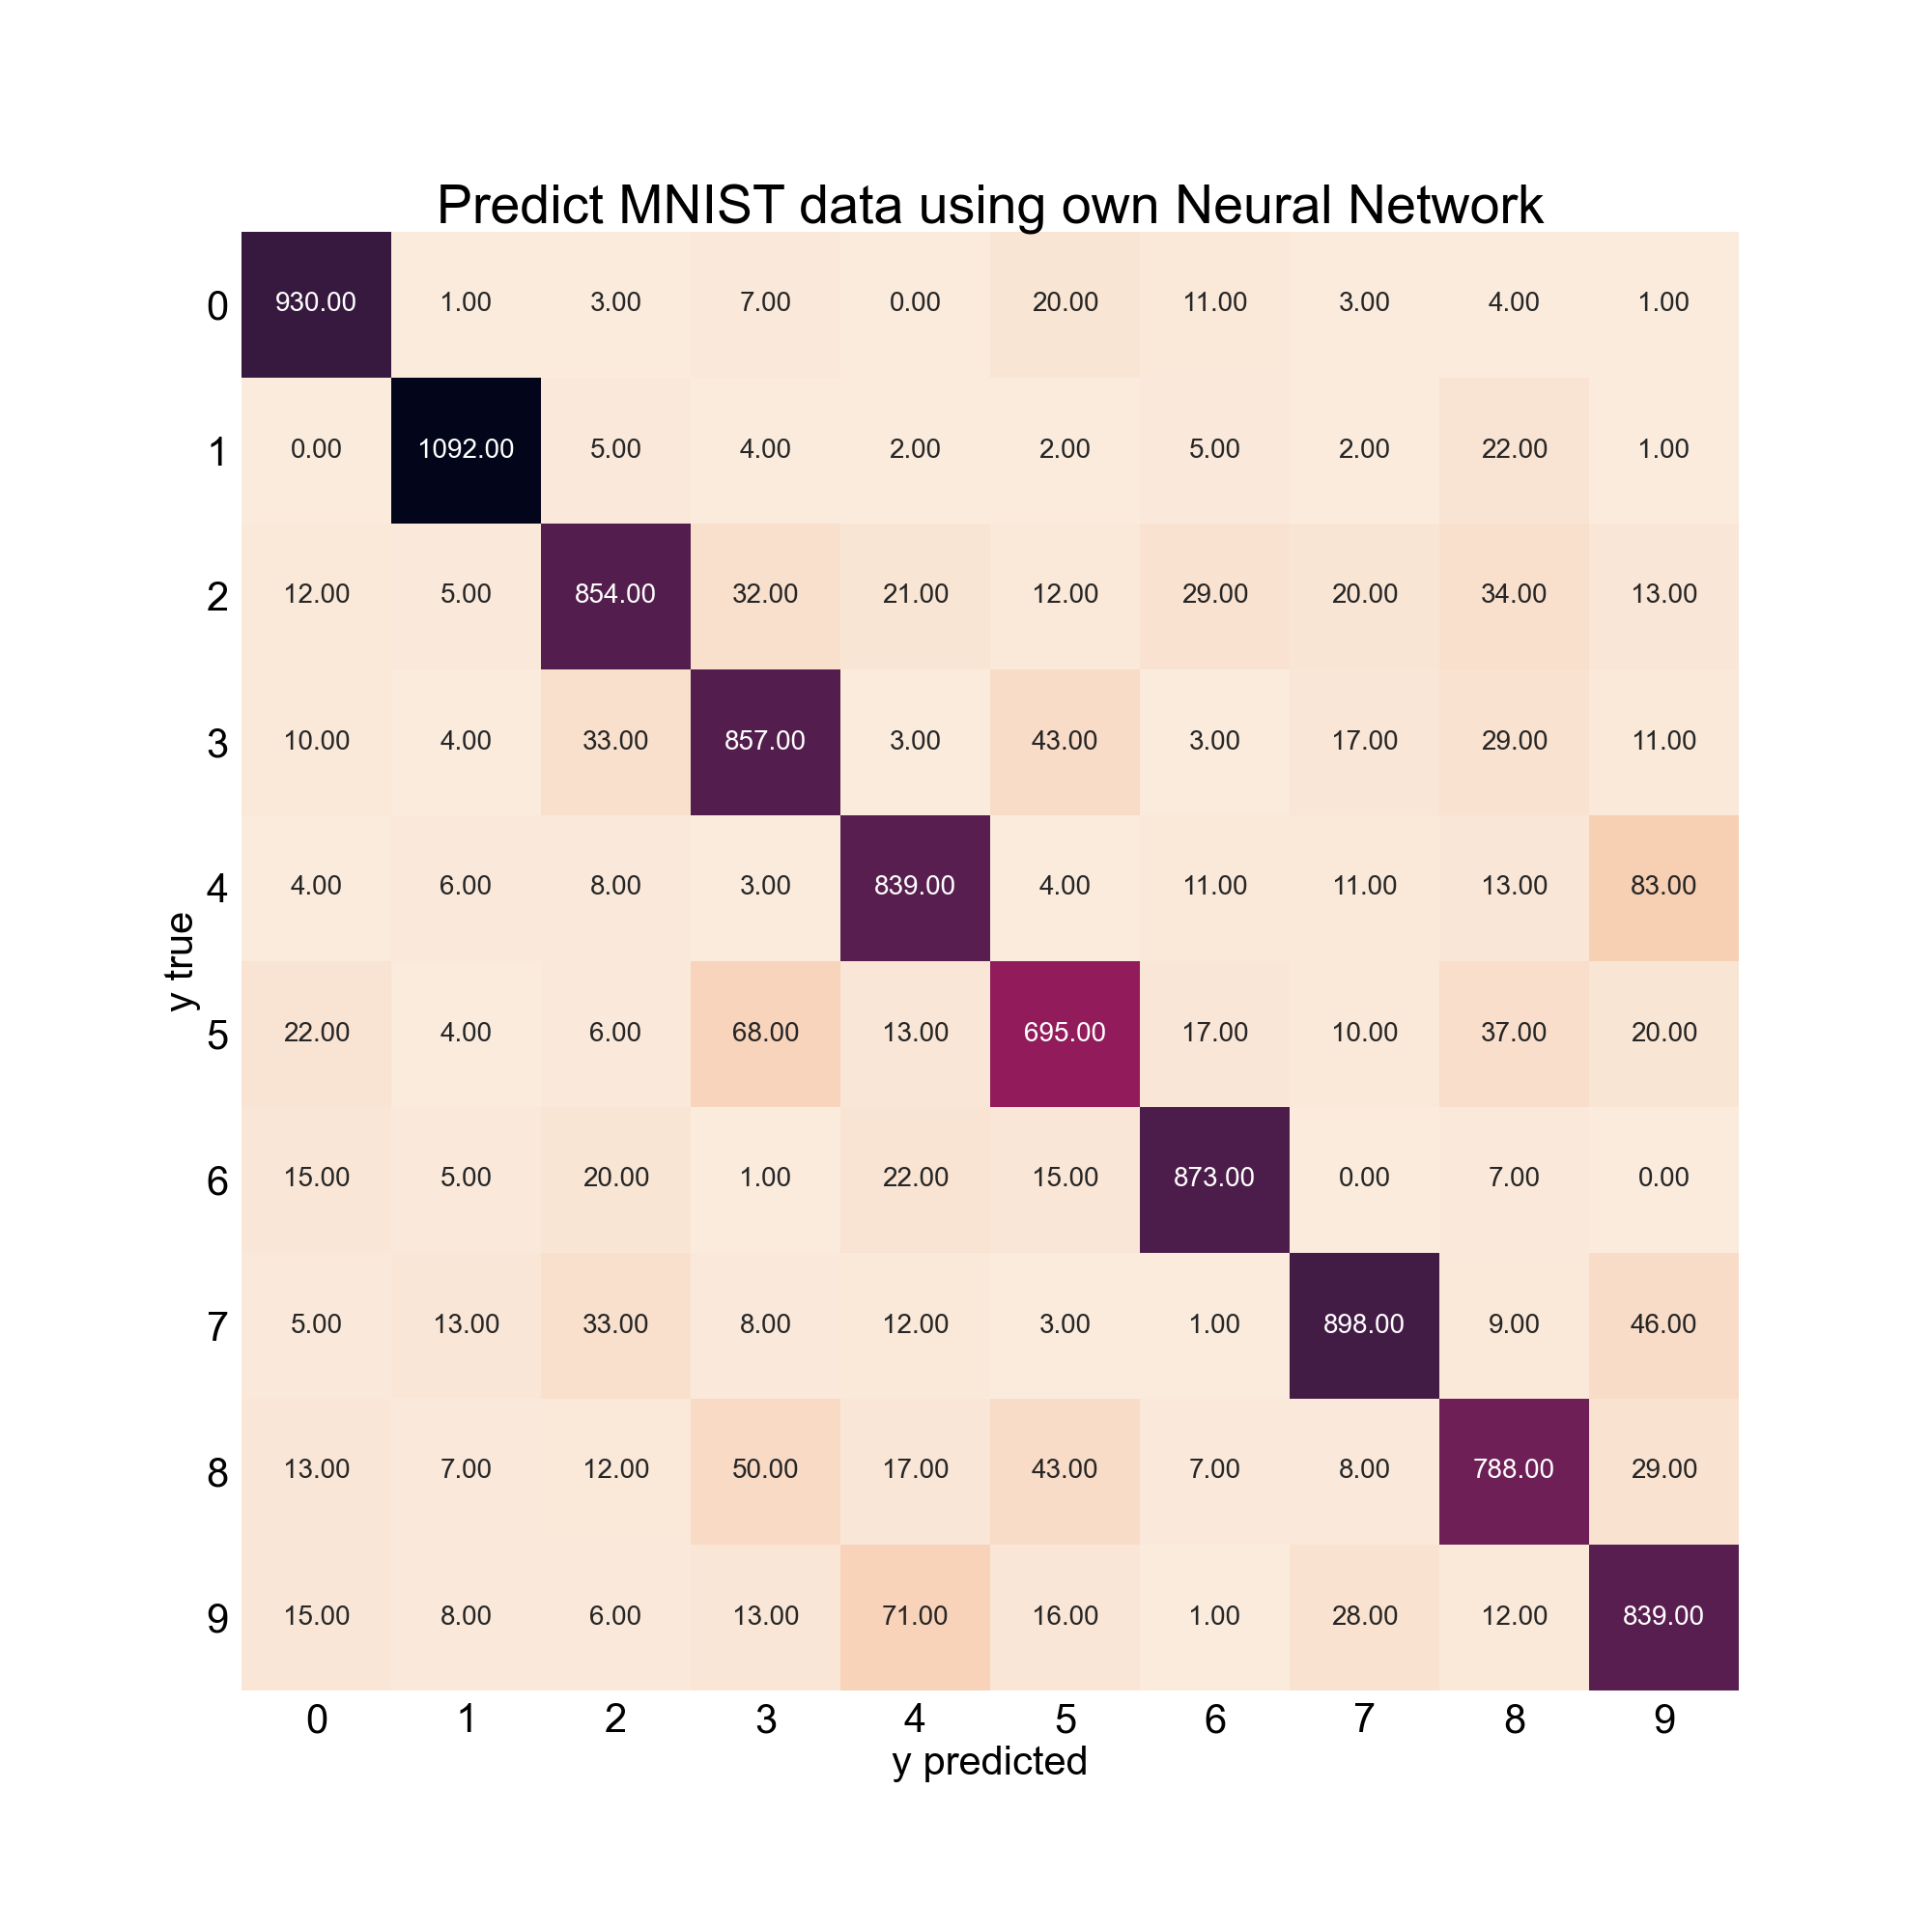
\includegraphics[width=7.9cm]{Figures/MNIST_confMatrix_ownNN.png}
\caption{Confusion matrix - Neural Network performing prediction on test set of MNIST data}
\label{fig:NN_mnist_confmatrix}
\end{figure}



\subsubsection{Classification of ECG data using Neural Network}
The ECG-featurizer \cite{bjorn-jostein_singstad_ecg-featurizer_nodate} managed to analyze 19609 out of 19635 of training data and 2203 out of 2203 of test data. The remaining 26 training data were taken out of the data set. Some NaN-values were also present in the training set. These were replaced by the mean of all the other values in the same category. 
Google Colab was used to do Bayesian optimization. Validation accuracy loss was used as the target to optimize the model.

\vspace{-4 mm}
\begin{table}[!htpb]
\vspace{4 mm}
\centerline{\begin{tabular}{lr} \hline\hline
Parameter                       & Values         \\ \hline
Learning rate   &  $1^{-5}, 1^{-4}, 1^{-3}, 0.01, 0.1$  \\
Batch size             & $10,20,30,...,100$               \\ 
Hidden layers           & $1,2,3,...,11$                \\  
Activation in hidden layers & ReLU, eLU, SeLU \\\hline\hline
\end{tabular}}
\caption{\label{tab:challenge_validation} Parameters used in the Bayesian optimization of the Neural Network used for classification of the PTB-XL ECG data.}
\end{table}

The accuracy score achieved on the test set proposed by the publisher of the PTB-XL ECG data was $0.415$
The conf matrix looks like this:

\subsection{Logistic regression}
\subsubsection{Classification of MNIST-data}
A subset of 1000 samples were used to grid search ([] $l2$-penalty and learning rate (constant) and then 2000 samples were used to train the model on the best parameters from the grid search.
\begin{figure}[htbp!]
%\centering
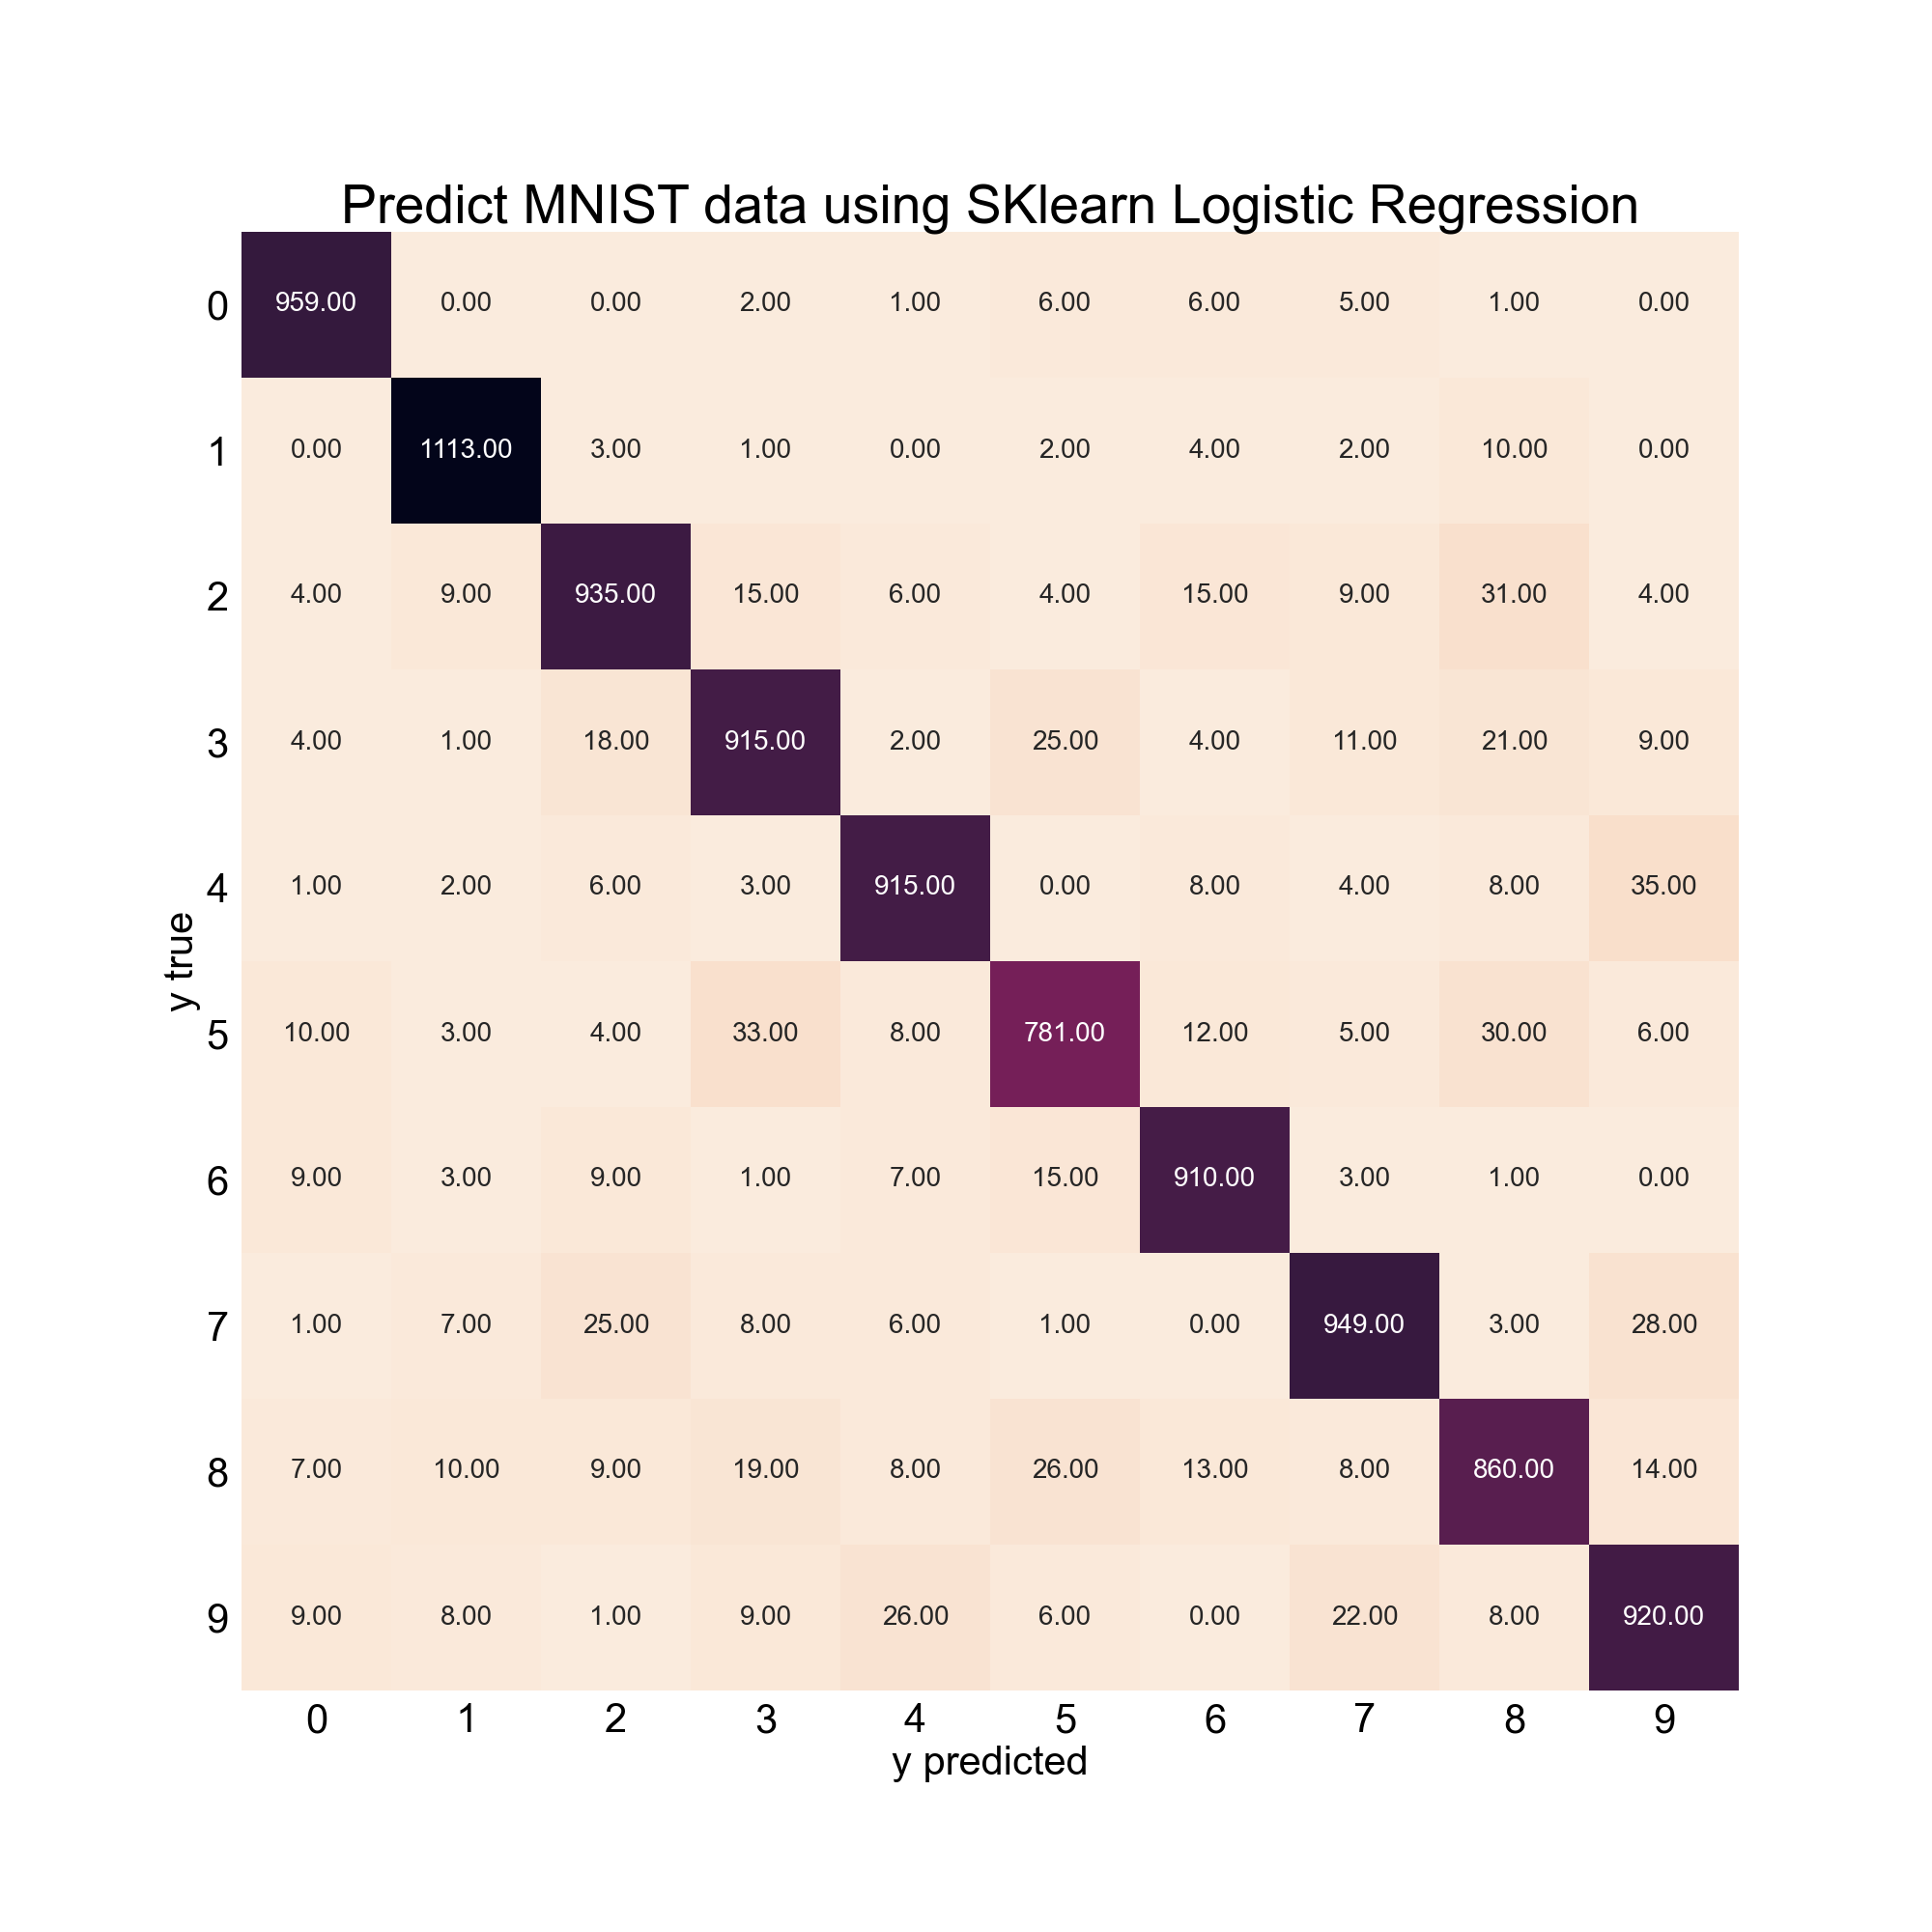
\includegraphics[width=7.9cm]{Figures/MNIST_confMatrix_sklearn_logreg.png}
\caption{LogReg }
\label{fig:OLS_ridge}
\end{figure}

\subsubsection{Classification of ECG-data}



Hold out validation

\subsubsection{Classify ECG data}

\section{Discussion}
The OLS SGD model that was developed from scratch was polynomial features. Compared to SKlearn it seems like this is not and alternative and maybe this does not work this way.


\textbf{Classification-MNIST}


\section{Conclusion}

\bibliographystyle{naturemag}
\bibliography{references}
\onecolumn
\appendix
%\section{Appendix}

\begin{figure}[htbp!]
\centering
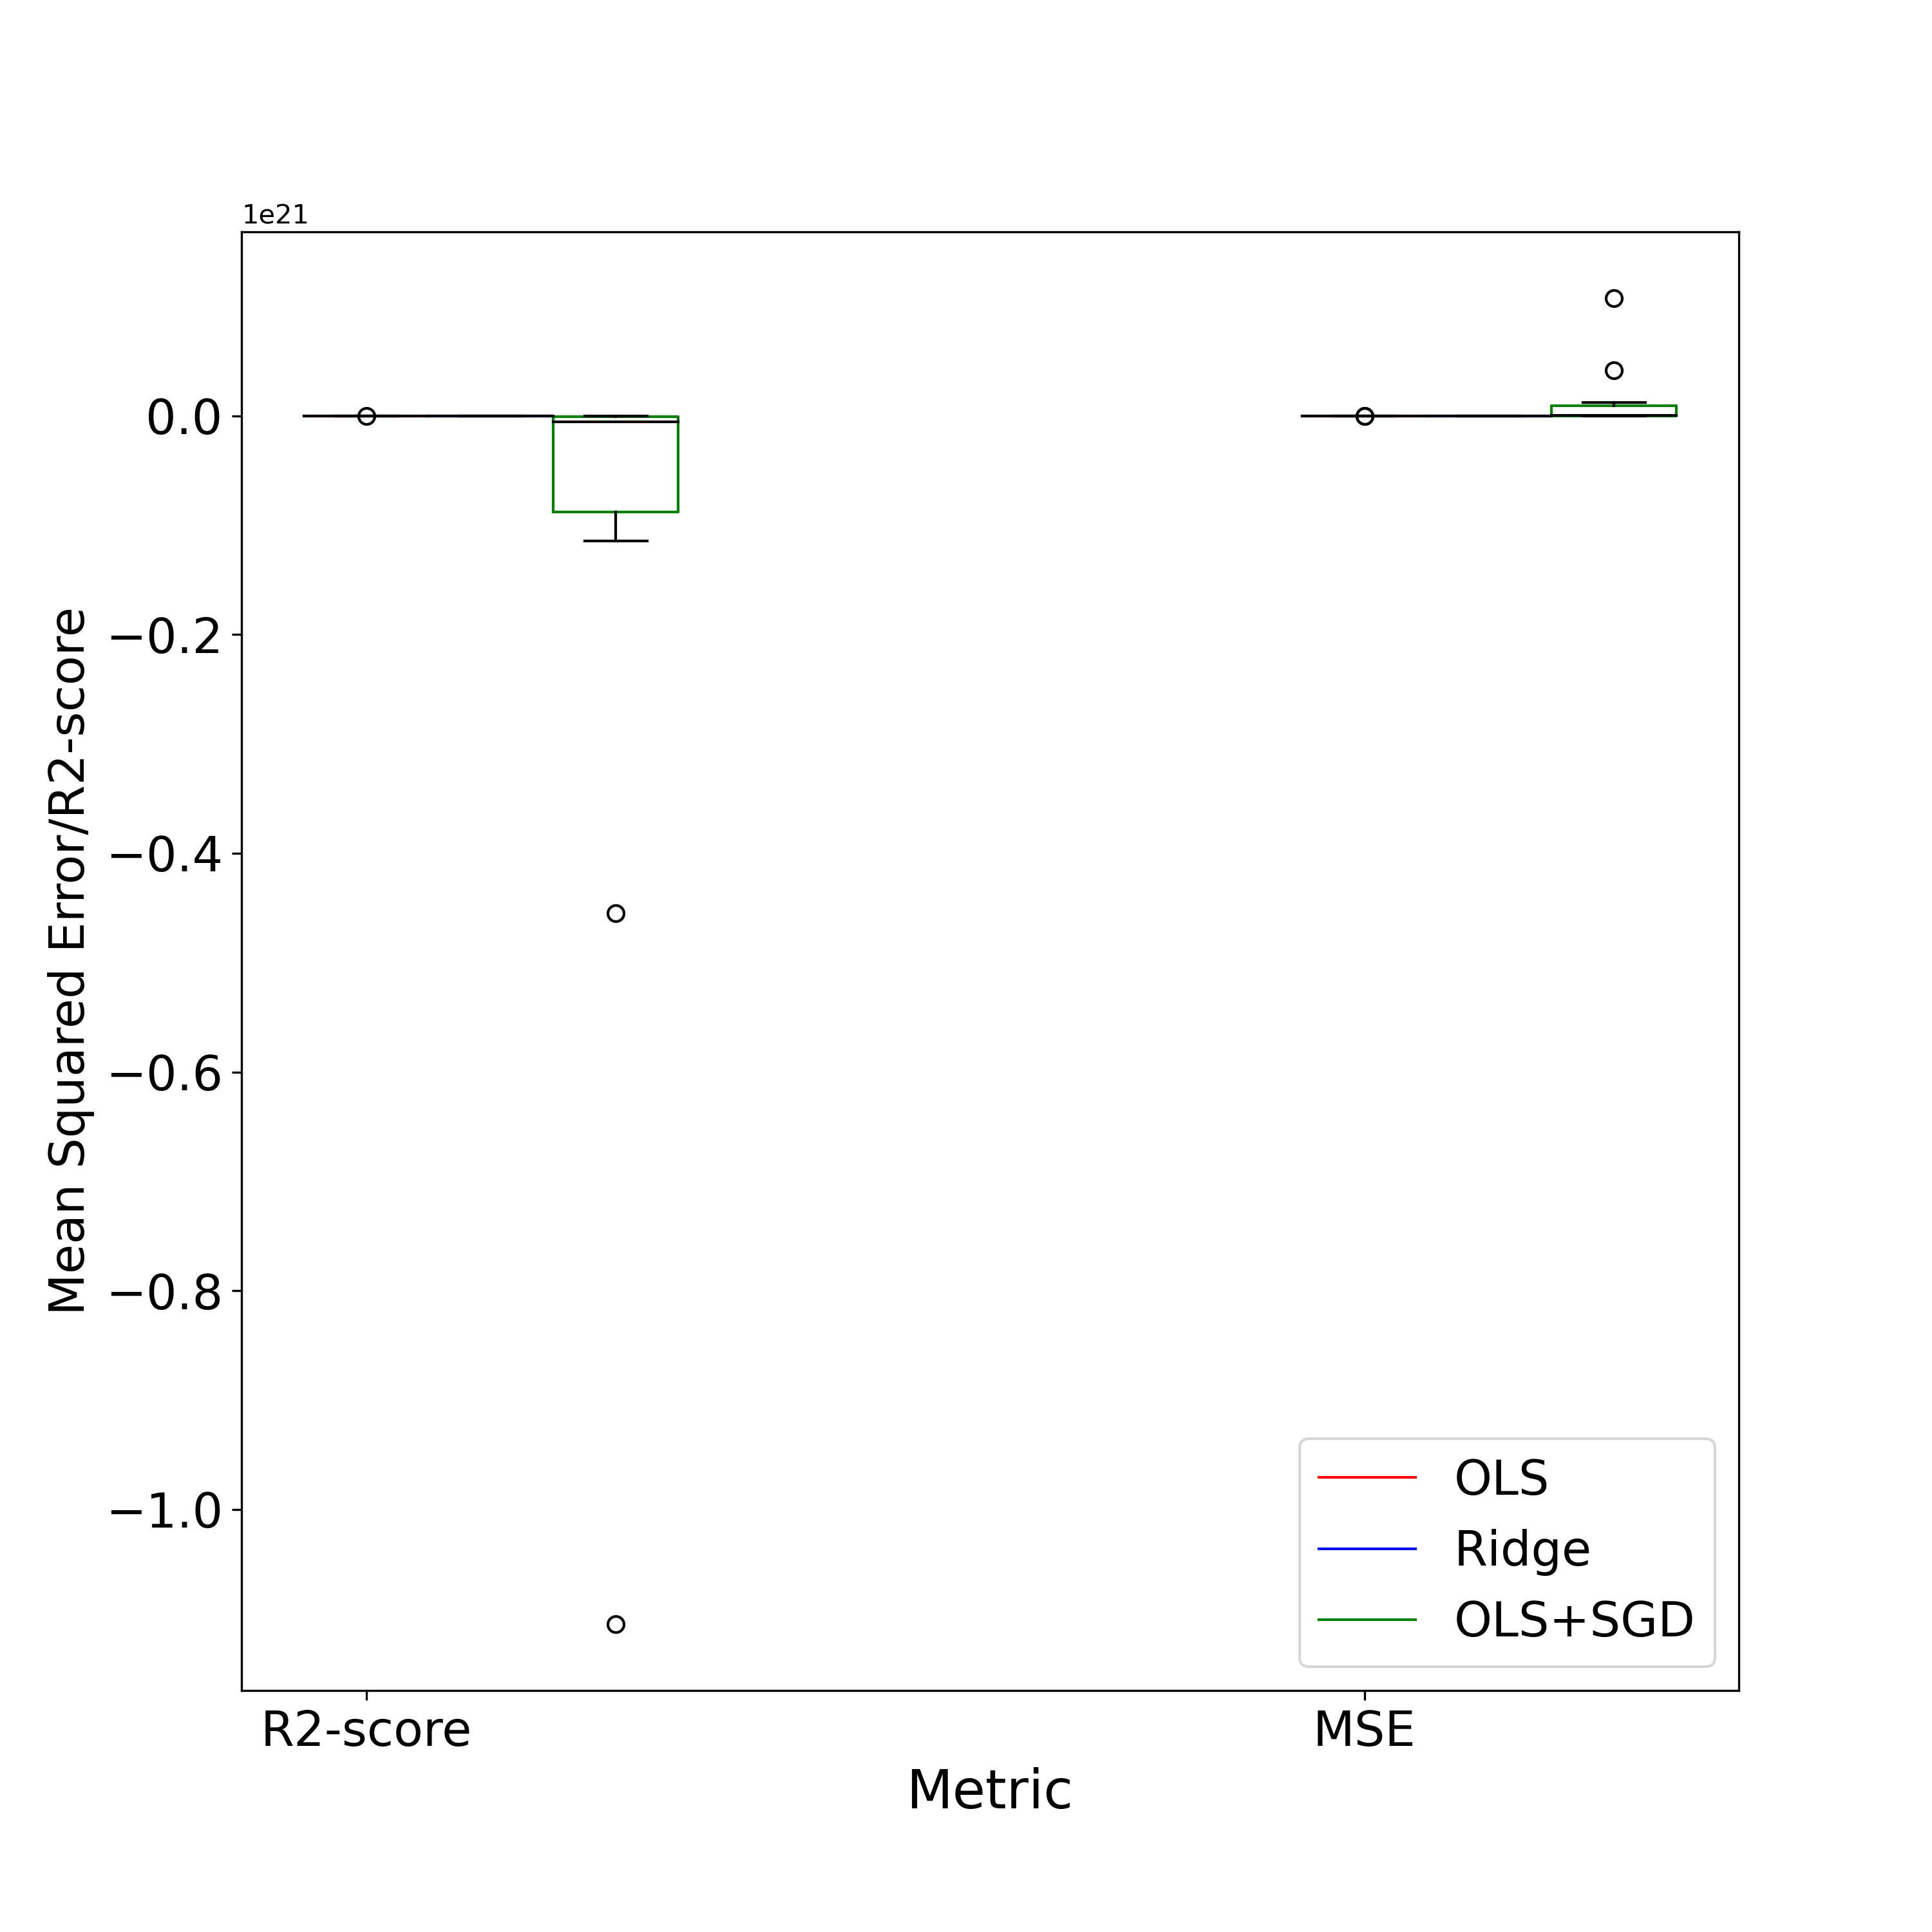
\includegraphics[width=0.65\textwidth]{Figures/boxplot_OLS_ridge_sgd.png}
\caption{R2-score and MSE score for a Ridge,OLS and OLS SGD model}
\label{fig:appendix_sdg}
\end{figure}

\end{document}

